\documentclass[a4paper,12pt,twoside]{memoir}

% Castellano
\usepackage[spanish,es-tabla]{babel}
\selectlanguage{spanish}
\usepackage[utf8]{inputenc}
\usepackage[T1]{fontenc}
\usepackage{lmodern} % scalable font
\usepackage{microtype}
\usepackage{placeins}

\RequirePackage{booktabs}
\RequirePackage[table]{xcolor}
\RequirePackage{xtab}
\RequirePackage{multirow}

% Links
\PassOptionsToPackage{hyphens}{url}\usepackage[colorlinks]{hyperref}
\hypersetup{
	allcolors = {red}
}

% Ecuaciones
\usepackage{amsmath}

% Rutas de fichero / paquete
\newcommand{\ruta}[1]{{\sffamily #1}}

% Párrafos
\nonzeroparskip

% Huérfanas y viudas
\widowpenalty100000
\clubpenalty100000

% Evitar solapes en el header
\nouppercaseheads

% Imagenes
\usepackage{graphicx}
\newcommand{\imagen}[2]{
	\begin{figure}[!h]
		\centering
		\includegraphics[width=0.9\textwidth]{#1}
		\caption{#2}\label{fig:#1}
	\end{figure}
	\FloatBarrier
}

\newcommand{\imagenflotante}[2]{
	\begin{figure}%[!h]
		\centering
		\includegraphics[width=0.9\textwidth]{#1}
		\caption{#2}\label{fig:#1}
	\end{figure}
}



% El comando \figura nos permite insertar figuras comodamente, y utilizando
% siempre el mismo formato. Los parametros son:
% 1 -> Porcentaje del ancho de página que ocupará la figura (de 0 a 1)
% 2 --> Fichero de la imagen
% 3 --> Texto a pie de imagen
% 4 --> Etiqueta (label) para referencias
% 5 --> Opciones que queramos pasarle al \includegraphics
% 6 --> Opciones de posicionamiento a pasarle a \begin{figure}
\newcommand{\figuraConPosicion}[6]{%
  \setlength{\anchoFloat}{#1\textwidth}%
  \addtolength{\anchoFloat}{-4\fboxsep}%
  \setlength{\anchoFigura}{\anchoFloat}%
  \begin{figure}[#6]
    \begin{center}%
      \Ovalbox{%
        \begin{minipage}{\anchoFloat}%
          \begin{center}%
            \includegraphics[width=\anchoFigura,#5]{#2}%
            \caption{#3}%
            \label{#4}%
          \end{center}%
        \end{minipage}
      }%
    \end{center}%
  \end{figure}%
}

%
% Comando para incluir imágenes en formato apaisado (sin marco).
\newcommand{\figuraApaisadaSinMarco}[5]{%
  \begin{figure}%
    \begin{center}%
    \includegraphics[angle=90,height=#1\textheight,#5]{#2}%
    \caption{#3}%
    \label{#4}%
    \end{center}%
  \end{figure}%
}
% Para las tablas
\newcommand{\otoprule}{\midrule [\heavyrulewidth]}
%
% Nuevo comando para tablas pequeñas (menos de una página).
\newcommand{\tablaSmall}[5]{%
 \begin{table}
  \begin{center}
   \rowcolors {2}{gray!35}{}
   \begin{tabular}{#2}
    \toprule
    #4
    \otoprule
    #5
    \bottomrule
   \end{tabular}
   \caption{#1}
   \label{tabla:#3}
  \end{center}
 \end{table}
}

%
%Para el float H de tablaSmallSinColores
\usepackage{float}

%
% Nuevo comando para tablas pequeñas (menos de una página).
\newcommand{\tablaSmallSinColores}[5]{%
 \begin{table}[H]
  \begin{center}
   \begin{tabular}{#2}
    \toprule
    #4
    \otoprule
    #5
    \bottomrule
   \end{tabular}
   \caption{#1}
   \label{tabla:#3}
  \end{center}
 \end{table}
}

\newcommand{\tablaApaisadaSmall}[5]{%
\begin{landscape}
  \begin{table}
   \begin{center}
    \rowcolors {2}{gray!35}{}
    \begin{tabular}{#2}
     \toprule
     #4
     \otoprule
     #5
     \bottomrule
    \end{tabular}
    \caption{#1}
    \label{tabla:#3}
   \end{center}
  \end{table}
\end{landscape}
}

%
% Nuevo comando para tablas grandes con cabecera y filas alternas coloreadas en gris.
\newcommand{\tabla}[6]{%
  \begin{center}
    \tablefirsthead{
      \toprule
      #5
      \otoprule
    }
    \tablehead{
      \multicolumn{#3}{l}{\small\sl continúa desde la página anterior}\\
      \toprule
      #5
      \otoprule
    }
    \tabletail{
      \hline
      \multicolumn{#3}{r}{\small\sl continúa en la página siguiente}\\
    }
    \tablelasttail{
      \hline
    }
    \bottomcaption{#1}
    \rowcolors {2}{gray!35}{}
    \begin{xtabular}{#2}
      #6
      \bottomrule
    \end{xtabular}
    \label{tabla:#4}
  \end{center}
}

%
% Nuevo comando para tablas grandes con cabecera.
\newcommand{\tablaSinColores}[6]{%
  \begin{center}
    \tablefirsthead{
      \toprule
      #5
      \otoprule
    }
    \tablehead{
      \multicolumn{#3}{l}{\small\sl continúa desde la página anterior}\\
      \toprule
      #5
      \otoprule
    }
    \tabletail{
      \hline
      \multicolumn{#3}{r}{\small\sl continúa en la página siguiente}\\
    }
    \tablelasttail{
      \hline
    }
    \bottomcaption{#1}
    \begin{xtabular}{#2}
      #6
      \bottomrule
    \end{xtabular}
    \label{tabla:#4}
  \end{center}
}

%
% Nuevo comando para tablas grandes sin cabecera.
\newcommand{\tablaSinCabecera}[5]{%
  \begin{center}
    \tablefirsthead{
      \toprule
    }
    \tablehead{
      \multicolumn{#3}{l}{\small\sl continúa desde la página anterior}\\
      \hline
    }
    \tabletail{
      \hline
      \multicolumn{#3}{r}{\small\sl continúa en la página siguiente}\\
    }
    \tablelasttail{
      \hline
    }
    \bottomcaption{#1}
  \begin{xtabular}{#2}
    #5
   \bottomrule
  \end{xtabular}
  \label{tabla:#4}
  \end{center}
}



\definecolor{cgoLight}{HTML}{EEEEEE}
\definecolor{cgoExtralight}{HTML}{FFFFFF}

%
% Nuevo comando para tablas grandes sin cabecera.
\newcommand{\tablaSinCabeceraConBandas}[5]{%
  \begin{center}
    \tablefirsthead{
      \toprule
    }
    \tablehead{
      \multicolumn{#3}{l}{\small\sl continúa desde la página anterior}\\
      \hline
    }
    \tabletail{
      \hline
      \multicolumn{#3}{r}{\small\sl continúa en la página siguiente}\\
    }
    \tablelasttail{
      \hline
    }
    \bottomcaption{#1}
    \rowcolors[]{1}{cgoExtralight}{cgoLight}

  \begin{xtabular}{#2}
    #5
   \bottomrule
  \end{xtabular}
  \label{tabla:#4}
  \end{center}
}




\graphicspath{ {./img/} }

% Capítulos
\chapterstyle{bianchi}
\newcommand{\capitulo}[2]{
	\setcounter{chapter}{#1}
	\setcounter{section}{0}
	\setcounter{figure}{0}
	\setcounter{table}{0}
	\chapter*{#2}
	\addcontentsline{toc}{chapter}{#2}
	\markboth{#2}{#2}
}

% Apéndices
\renewcommand{\appendixname}{Apéndice}
\renewcommand*\cftappendixname{\appendixname}

\newcommand{\apendice}[1]{
	%\renewcommand{\thechapter}{A}
    \chapter{#1}
}

\renewcommand*\cftappendixname{\appendixname\ }

% Formato de portada
\makeatletter
\usepackage{xcolor}
\newcommand{\tutor}[1]{\def\@tutor{#1}}
\newcommand{\course}[1]{\def\@course{#1}}
\definecolor{cpardoBox}{HTML}{E6E6FF}
\def\maketitle{
  \null
  \thispagestyle{empty}
  % Cabecera ----------------
\noindent
\includegraphics[width=\textwidth]{cabecera}\vspace{1cm}%
  \vfill
  % Título proyecto y escudo informática ----------------
  \colorbox{cpardoBox}{%
    \begin{minipage}{.8\textwidth}
      \vspace{.5cm}\Large
      \begin{center}
      \textbf{TFG del Grado en Ingeniería Informática}\vspace{.6cm}\\
      \textbf{\LARGE\@title{}}
      \end{center}
      \vspace{.2cm}
    \end{minipage}

  }%
  \hfill\begin{minipage}{.20\textwidth}
    
\includegraphics[width=\textwidth]{escudoInfor}
  \end{minipage}
  \vfill
  % Datos de alumno, curso y tutores ------------------
  \begin{center}%
  {%
    \noindent\LARGE
    Presentado por \@author{}\\ 
    en Universidad de Burgos --- \@date{}\\
    Tutor: \@tutor{}\\
  }%
  \end{center}%
  \null
  \cleardoublepage
  }
\makeatother


% Datos de portada
\title{Mixing Models \\Documentación Técnica}
\author{Humberto Marijuán Santamaría}
\tutor{Luis Rodrigo Izquierdo Millán}
\tutor{José Manuel Galán Ordax}
\date{\today}

\begin{document}

\maketitle



\cleardoublepage



%%%%%%%%%%%%%%%%%%%%%%%%%%%%%%%%%%%%%%%%%%%%%%%%%%%%%%%%%%%%%%%%%%%%%%%%%%%%%%%%%%%%%%%%



\frontmatter


\clearpage

% Indices
\tableofcontents

\clearpage

\listoffigures

\clearpage

\listoftables

\clearpage

\mainmatter

\appendix

\apendice{Plan de Proyecto Software}

\section{Introducción}

En este apéndice se ha recogido la planificación temporal, estudio de viabilidad y viabilidad legal.

\section{Planificación temporal}

Para realizar la planificación temporal se ha utilizado la metodología de gestión ágil de proyectos (Scrum). La planificación del proyecto se realizó desde GitHub junto con la extensión Zenhub. En estas herramientas de gestión de versiones se realizaron varios sprints de trabajo con una duración aproximada de 2 semanas. En estos periodos de tiempo se han definido tareas a completar. 

Estas tareas o \textit{issues} están asignadas a una persona, tienen una etiqueta de cara a su organización y una estimación de la dificultad. En cuanto a las etiquetas o labels, en este proyecto se han trabajado con las predefinidas por GitHub siendo estas:
\begin{itemize}
    \item \textbf{Enhacement:} Añade una nueva característica o petición. Se puede ver con mayor detalle en \href{https://github.com/humbertoms99/Mixing_models/issues?q=label%3Aenhancement+}{Enhacement}.
    \item \textbf{Bug:} Corrección de errores o funcionamientos incorrectos de la aplicación. Se puede ver con mayor detalle en \href{https://github.com/humbertoms99/Mixing_models/issues?q=label%3Abug+}{Bug}.
    \item \textbf{Documentation:} Tareas de documentación, en las que se espera añadir o mejorar documentos. Se puede ver con mayor detalle en \href{https://github.com/humbertoms99/Mixing_models/issues?q=label%3Adocumentation}{Documentation}.  
    \item \textbf{Duplicate:} Referentes a issues ya existentes.
    \item \textbf{Good first issue:} Tareas para facilitar el uso a nuevos usuarios. Se puede ver con mayor detalle en  \href{https://github.com/humbertoms99/Mixing_models/issues?q=label%3A%22good+first+issue%22}{Good first issue}.
    \item \textbf{Help wanted:} Tareas que requieren ayuda externa.
    \item \textbf{Invalid:} Tareas incorrectas.
    \item \textbf{Question:} Se solicita más información.
    \item \textbf{Wontfix:} Tareas que no han sido resueltas o que no están funcionando en ese momento.
\end{itemize}

\subsection{Sprints del proyecto}

Antes de comenzar con el desarrollo de funcionalidades para la aplicación se realizaron algunas tareas previas como: decisión de lenguajes con los que trabajar, herramientas a utilizar y un periodo de formación.

Antes de empezar con cualquier desarrollo se realizó un curso de \LaTeX (Más información en la issue \href{https://github.com/humbertoms99/Mixing_models/issues/1}{Curso de para aprender a usar Latex}) con el objetivo de poder documentar a la vez que se añadían funcionalidades. A continuación, se realizaron algunas tareas de análisis de la herramienta GitHub para comprender en profundidad sus posibilidades. Se leyeron algunos artículos sobre las \href{https://github.com/humbertoms99/Mixing_models/issues/2}{\textit{Milestones} y \textit{Sprints}}, junto con una aproximación a los \href{https://github.com/humbertoms99/Mixing_models/issues/3}{\textit{GitHub Reports}}.

También se preparó el entorno de desarrollo, descargando algunas herramientas como: Instalación Visual Studio Code y configuración extensiones para trabajar con Angular, Postman, extensión de ZenHub, Debian y Mendeley inicialmente.

\subsubsection{Sprints análisis}

Previo al desarrollo de funcionalidades se lleva a cabo una etapa de análisis. Durante estas semanas se realizó un análisis en profundidad del artículo \textit{Using n-alkanes to estimate diet composition of herbivores} \cite{problemn-alkanes2007}. Durante este periodo se aprendió sobre cómo resolver sistemas de ecuaciones con restricciones. Se resolvieron ejercicios en Matlab para entender aun más en profundidad los pasos para resolver estos sistemas. 

Una vez se definió y entendió el problema planteado se realizó una búsqueda de librerías y lenguajes para desarrollar posteriormente la aplicación.  

\subsubsection{Sprints iniciales}

Durante los primeros meses se realizó la instalación de la librería GLPK \cite{glpk:package} y se realizaron algunos ejemplos para llamar desde una proyecto front a una API que realizara funcionalidades de la librería, en concreto resolviera problemas de programación lineal, y recibiéramos esos resultados desde el proyecto front. 

\subsubsection{Sprint: 17 Mayo - 31 Mayo, 2022}

Una vez se conectaron los dos proyectos se empezaron a desarrollar de forma simultánea tanto la API como el front, utilizando la herramienta Postman para hacer pruebas de peticiones.

Este sprint se centró en realizar un flujo en el cual se introducían los datos desde el front y por medio de una petición al API escrita en laravel se recibía la respuesta al problema. A partir de la cual se hizo una primera visual de los resultados.

Las tareas completadas son representadas en el gráfico de la figura \ref{fig:sprint_17_31_may}.

\begin{itemize}
    \item \textbf{\#4-Resolver problemas Non-negative least square, min y max desde api laravel}.
    \item \textbf{\#5-Realizar ciclo de recepción y mostrar los resultados desde la web}.
    \item \textbf{\#6-Subida documentación y códigos}.
\end{itemize}

\begin{figure}[h!] 
\centering
    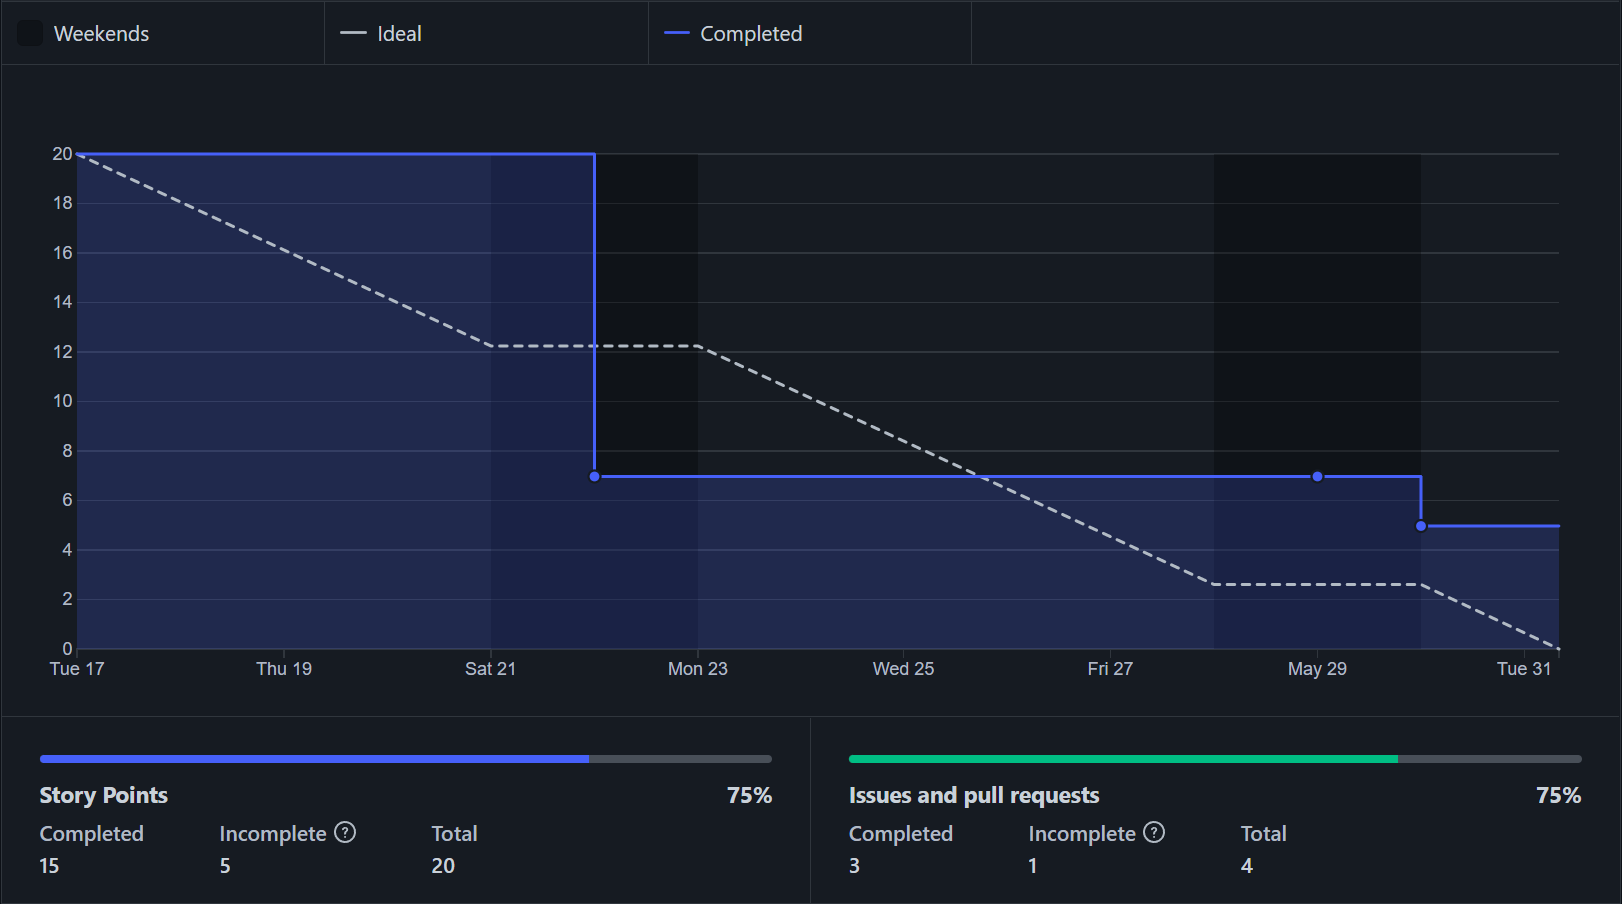
\includegraphics[width=0.8\textwidth]{img/sprint_17_31_may.PNG}
\caption{Sprint: 17 Mayo - 31 Mayo, 2022}
\label{fig:sprint_17_31_may}
\end{figure}

\newpage

\subsubsection{Sprint: 31 Mayo - 14 Junio, 2022}

Este sprint se centró principalmente en preparar los documentos para importar y exportar, preparando también todo el sistema de carga de archivos de la web. Además de configurar los ficheros de traducciones en la web.

\begin{itemize}
    \item \textbf{\#7-Funcionamiento paquete GLPK}.
    \item \textbf{\#8-Alert proyección no coincidente con punto}.
    \item \textbf{\#9-Exports solución y datos problemas}.
    \item \textbf{\#10-Descargar .mod de cada elemento de la solución}.
    \item \textbf{\#11-Import datos problema}.
    \item \textbf{\#12-Sistema de Traducciones}.
    \item \textbf{\#14-Export csv traducidos}.
\end{itemize}

Podemos ver el gráfico correspondiente a las tareas anteriores en la figura \ref{fig:sprint_31_14_jun}.

\begin{figure}[h!] 
\centering
    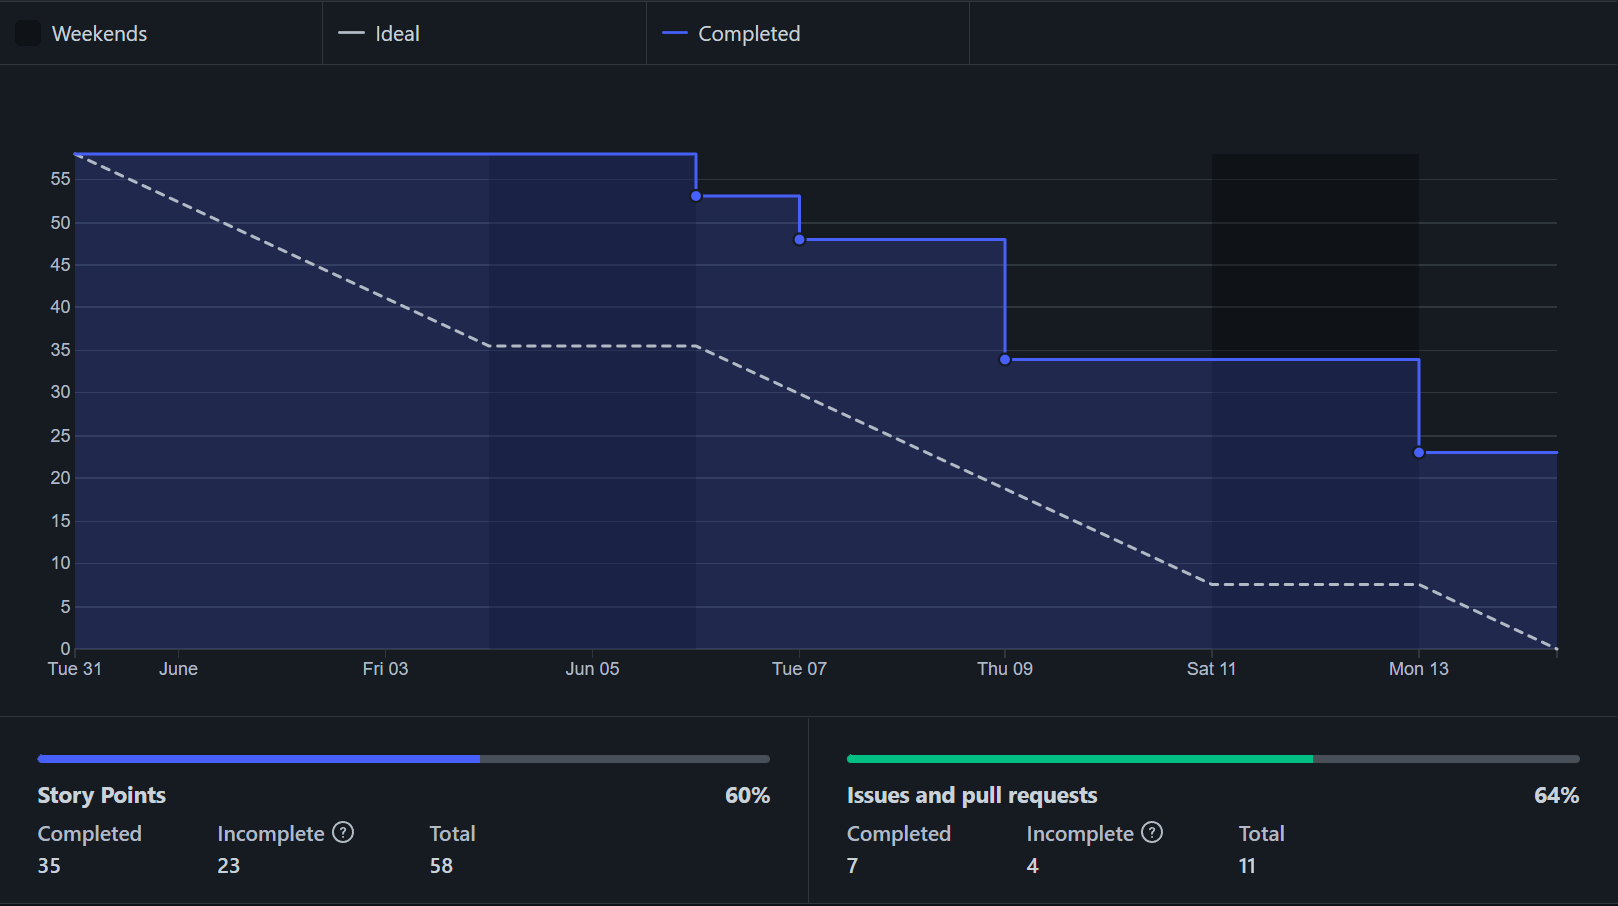
\includegraphics[width=0.8\textwidth]{img/sprint_31_14_jun.PNG}
\caption{Sprint: 31 Mayo - 14 Junio, 2022}
\label{fig:sprint_31_14_jun}
\end{figure}

\subsubsection{Sprint: 14 Junio - 28 Junio, 2022}

Este Sprint está marcado principalmente por la subida a un servidor de nuestro proyecto, aunque también se hicieron pequeños ajustes de maquetación y procedimientos de cara a agilizar el uso de la aplicación

\begin{itemize}
    \item \textbf{\#13-Slider web}.
    \item \textbf{\#15-Ajustes maquetación solución}.
    \item \textbf{\#16-Subida a servidor}.
    \item \textbf{\#17-Función reset arrays}.
    \item \textbf{\#19-Añadir línea min max en exports solución}.
\end{itemize}

Podemos ver el gráfico \textit{"Burndown report"} correspondiente al sprint en la figura \ref{fig:sprint_14_28_jun}.

\begin{figure}[h!] 
\centering
    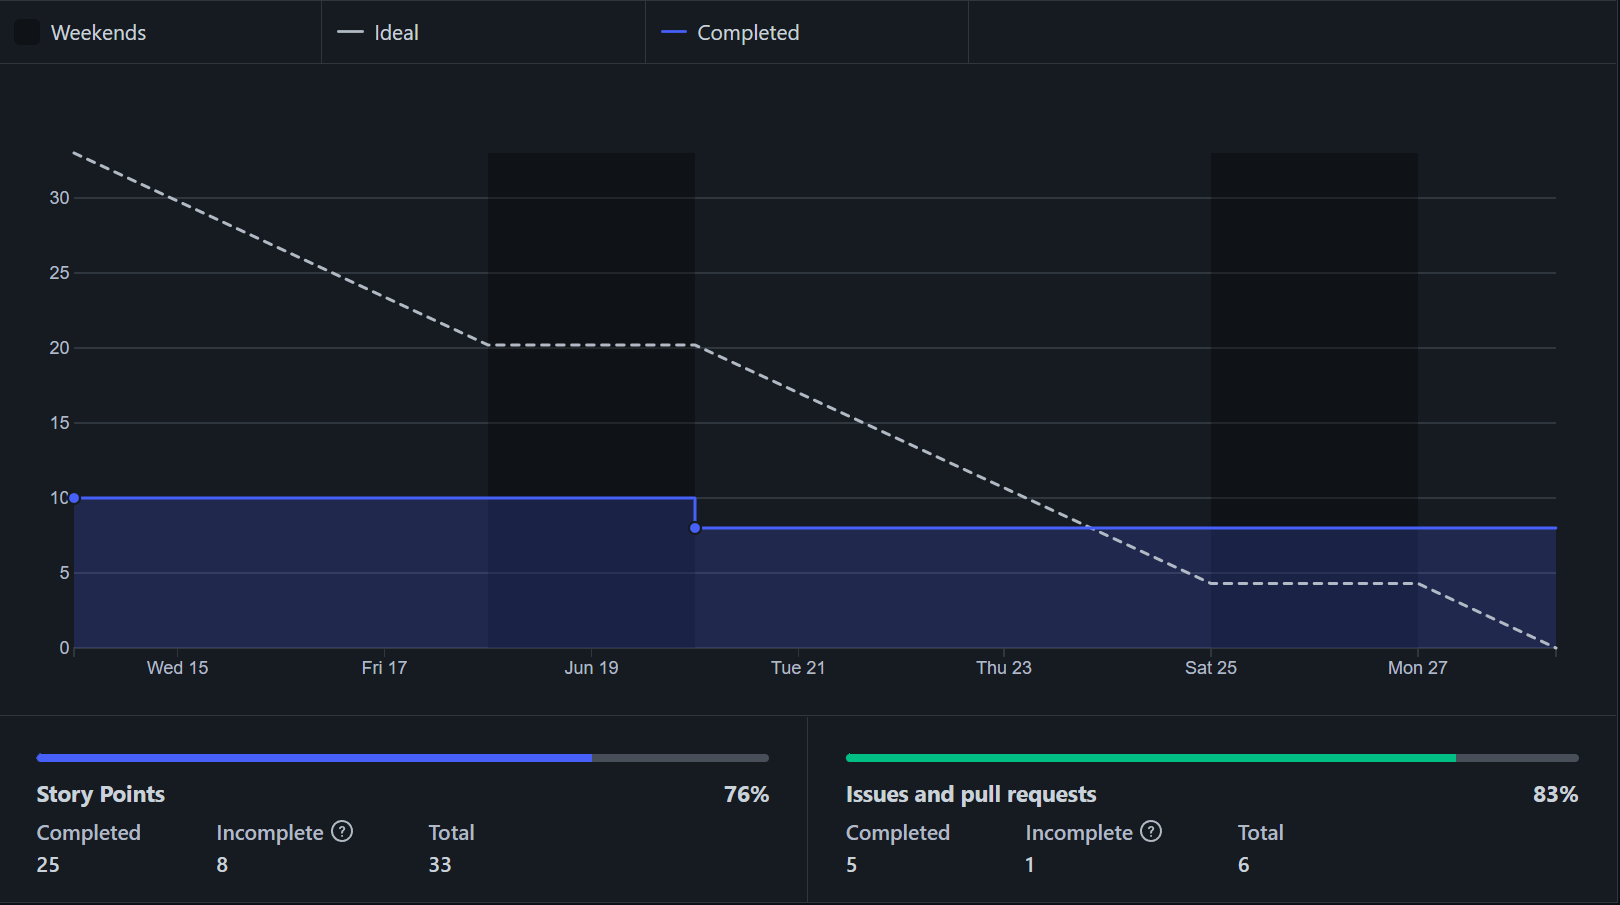
\includegraphics[width=0.8\textwidth]{img/sprint_14_28_jun.PNG}
\caption{Sprint: 14 Mayo - 28 Junio, 2022}
\label{fig:sprint_14_28_jun}
\end{figure}

\newpage
\subsubsection{Sprint: 6 Septiembre - 20 Septiembre, 2022}

En este último sprint se han añadido cambios para adaptar por completo las funciones a la nueva librería, se han resuelto algunos bugs, y se ha realizado la primera versión de los documentos memoria y anexos.

\begin{itemize}
    \item \textbf{\#18-Primera versión memoria}
    \item \textbf{\#23-Búsqueda funciones resuelvan las funciones usadas en el API}
    \item \textbf{\#24-Cambio función api "deleteAllfiles()" al proyecto front}
    \item \textbf{\#25-Cambio función API - "getTextFiles()" al proyecto front}
    \item \textbf{\#26-Cambio función API - "downloadFile()" al proyecto front}
    \item \textbf{\#28-Cambio título web}
    \item \textbf{\#29-Error recargar la página al cambiar de idioma}
    \item \textbf{\#30-Primera versión documento anexos}
    \item \textbf{\#32-Redondeo proyecciones a tres decimales}
    \item \textbf{\#33-Cargar archivo y darle a crear se queda nombre archivo}
    \item \textbf{\#34-Correción refresh web netlify}
\end{itemize}

Podemos ver el gráfico correspondiente a las tareas anteriores en la figura \ref{fig:sprint_06_20_sep}.

\begin{figure}[h!] 
\centering
    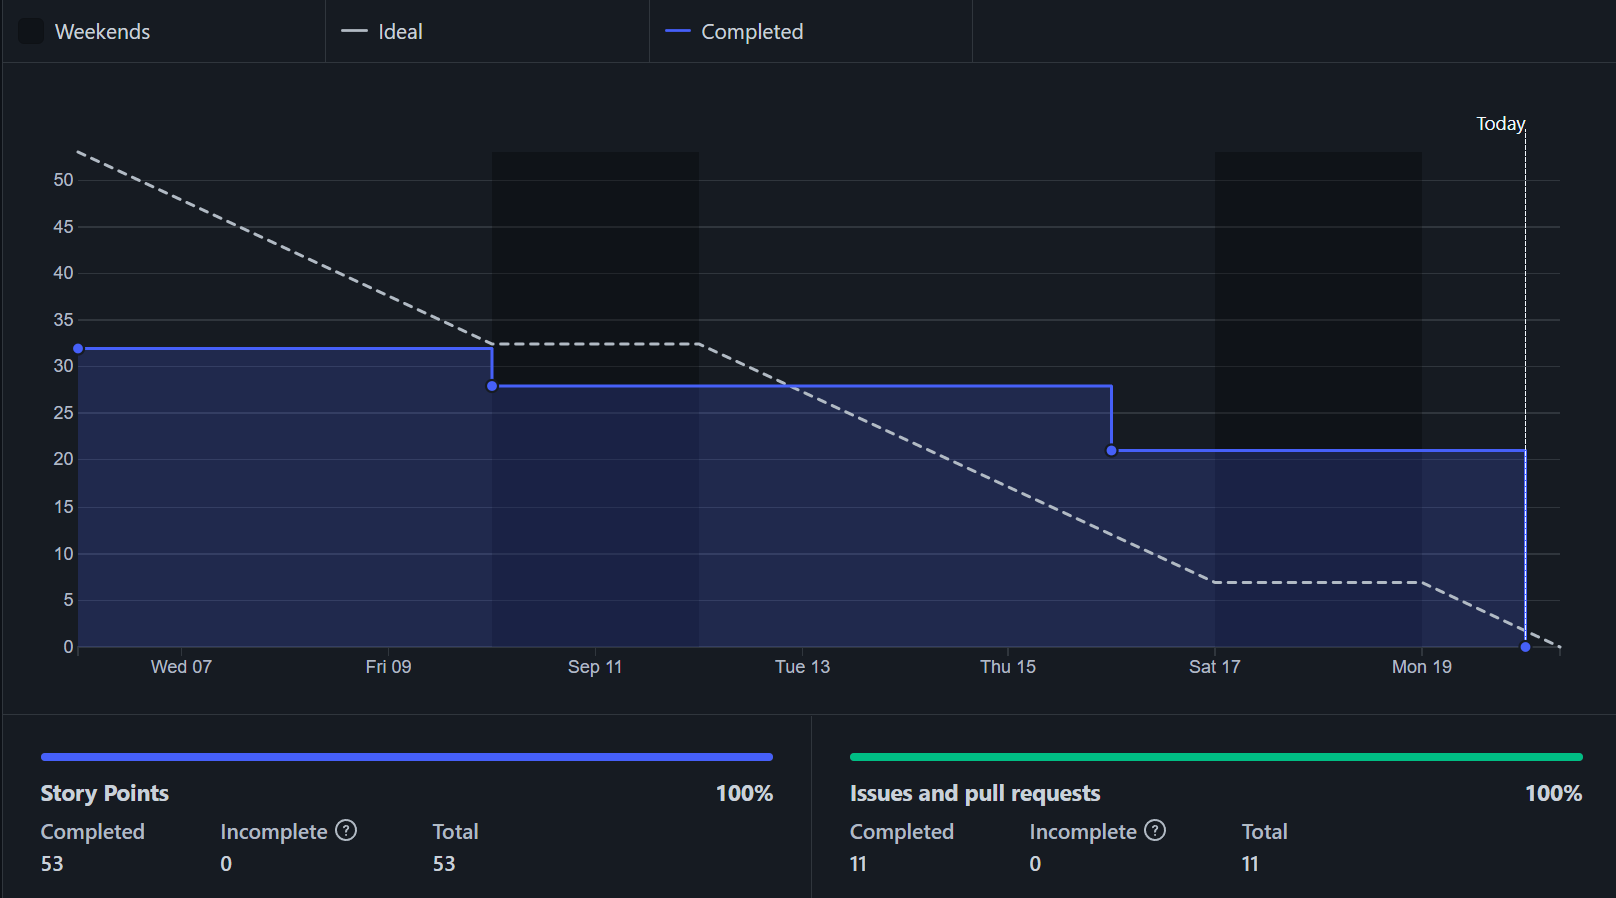
\includegraphics[width=0.8\textwidth]{img/sprint_06_20_sep.PNG}
\caption{Sprint: 06 Septiembre - 20 Septiembre, 2022}
\label{fig:sprint_06_20_sep}
\end{figure}

\section{Estudio de viabilidad}

En esta sección vamos a realizar un estudio de la viabilidad del proyecto tanto en el ámbito económico dando una aproximación de cuál sería la cantidad a pagar por un empresario, como de la viabilidad legal.

\subsection{Viabilidad económica}

De cara a la viabilidad económica vamos a centrarnos únicamente en el gasto que ha significado este proyecto, y no en el posible beneficio que podría dar. Para ello dividiremos los costes en cuatro:

\begin{itemize}
    \item Costes análisis
    \item Costes desarrollo
    \item Costes software
    \item Costes Hardware
\end{itemize}

\subsubsection{Costes análisis}

En cuanto a los costes de análisis en este proyecto solo ha trabajado un único analista web, que según Indeed \cite{indeed:oficial} el sueldo medio de un analista programador en España es de 28 350 € al año. Lo que estimaría una tarifa media de \textbf{19,68 €} por hora (28 350 / (30 horas x 48 semanas). Se han dedicado 10 semanas (estas semanas han sido en su mayoría antes de empezar el desarrollo, pero se han requerido algunos periodos temporales de análisis durante el desarrollo, ya cuantificados en esas 10 semanas)  al análisis del proyecto con jornadas de 6 horas diarias, es decir, unas 30 horas semanales.

30 horas/semana x 10 semanas x 19,68€/hora = \textbf{5 904 €} total

A este salario habría que añadirle los impuestos por seguridad social que actualmente aplicarían:

\begin{itemize}
    \item 23.6\% \textbf{contingencias comunes}.
    \item 5.5\% \textbf{tipo general de desempleo para contrato indefinido}.
    \item 0.20\% \textbf{FOGASA} (Fondo de Garantía Salarial).
    \item 0.60\% para \textbf{formación profesional}.
\end{itemize}

Estos datos (figuras \ref{fig:segsocial_contin} y \ref{fig:segsocial_otros}) provienen de la página de la Seguridad Social \cite{seguridad:social}, en el apartado de \textit{Régimen General de la Seguridad Social}.

\begin{figure}[h!] 
\centering
    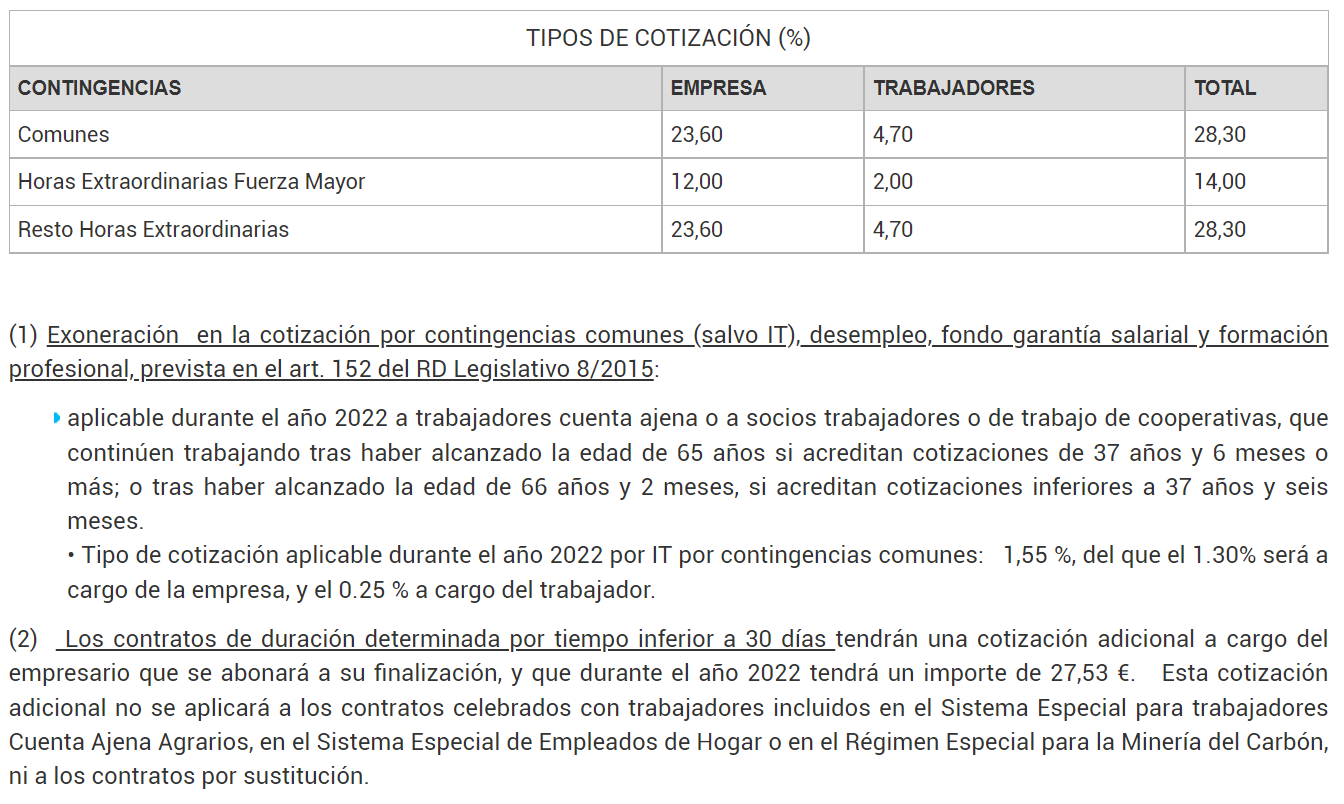
\includegraphics[width=0.8\textwidth]{img/seguridadsocial_1.PNG}
\caption{Régimen General de la Seguridad Social - Impuestos por contingencias comunes}
\label{fig:segsocial_contin}
\end{figure}

\begin{figure}[h!] 
\centering
    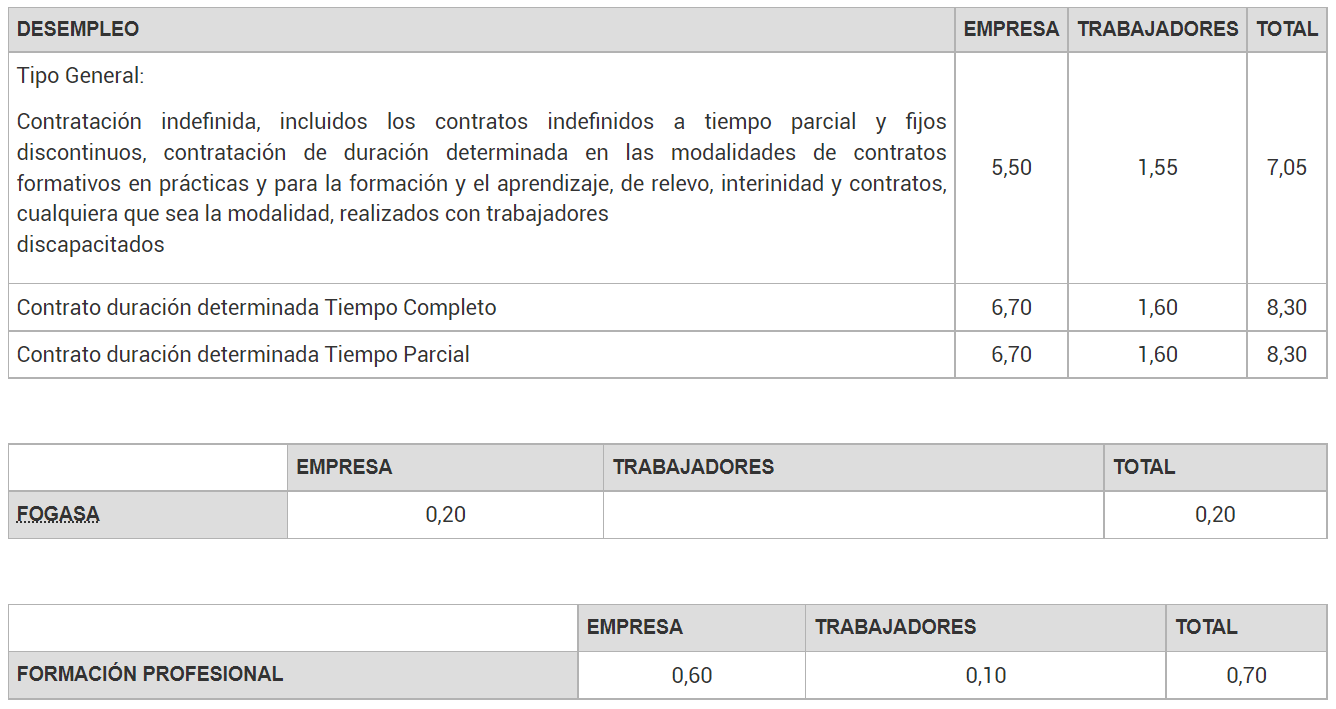
\includegraphics[width=0.8\textwidth]{img/seguridadsocial_2.PNG}
\caption{Régimen General de la Seguridad Social - Impuestos por otros}
\label{fig:segsocial_otros}
\end{figure}

El empleador debería añadir estos impuestos al total de pago tanto en la parte de desarrollo como de análisis.

$$ 5\:904 * (1 + 0,236 + 0,055 + 0,002 + 0,006) = \textbf{7 669, 296 €} $$


\subsubsection{Costes desarrollo}

En cuanto a los costes de desarrollo en este proyecto solo ha trabajado un único desarrollador web, que según Indeed \cite{indeed:oficial} el sueldo medio de desarrollador web en España es de 25 822 € al año. Lo que estimaría una tarifa media de \textbf{17,93 €} por hora (25 822 / (30 horas x 48 semanas). El proyecto se ha desarrollado en 5 periodos de 2 semanas con unas 6 horas al día, es decir, unas 30 horas semanales. 

30 horas/semana x (5 periodos x 2 semanas de duración) x 17,93€/hora = \textbf{5 379 €} (total trabajador sin impuestos)

Al igual que en el apartado anterior aplicamos los impuestos por seguridad social:

$$ 5\:379 \cdot (1 + 0,236 + 0,055 + 0,002 + 0,006) = \textbf{6 987,321 €} $$


\subsubsection{Costes software}

Las herramientas utilizadas son totalmente gratuitas. Por lo que no hay coste en este apartado. 

\subsubsection{Costes hardware}

El proyecto se ha desarrollado en un portátil Huawei KLVL-WXX9 con AMD Ryzen 7 4800h y 16GB de RAM con un precio de 700€ en enero de 2022. Partiendo que Hacienda marca que la amortización de ordenadores es de un 26\% multiplicado por 0,75 ( 11 meses de uso de noviembre 2021 a septiembre 2022, menos 2 meses de no trabajo da 9 meses de trabajo entre 12 que tiene el año da 0,75 siendo los meses de uso del portátil en un año) el portátil amortizado significaría una cantidad de 700 x 26\% = 182 al año, multiplicado por 0,75 = \textbf{136,5} seria el gasto en la duración de este proyecto.

Los gastos totales por tanto de este proyecto vienen representados en tabla de costes de la figura \ref{fig:costes_totales}.

\begin{table}[h]
    \centering
    \begin{tabular}{l c}
         \textbf{Tipo de Costes} & \textbf{Total } \\ 
         \hline
         \textit{Análisis} & 7 669, 296 € \\ 
         \textit{Desarrollo} & 6 987,321 € \\  
         \textit{Software} & 0 € \\ 
         \textit{Hardware} & 136,5 €   \\ 
         \hline
         \textbf{Total} & \textbf{14 793,117 €}\\ 
    \end{tabular}
    \caption{Tabla costes totales}
    \label{fig:costes_totales}
\end{table}


\subsection{Viabilidad legal}

Las herramientas utilizadas en el desarrollo del proyectos disponen de licencias gratuitas o son open source. En la tabla \ref{fig:herramientaslicense}  se muestra las licencias de cada herramientas utilizada.

\newpage

\begin{table}[h]
    \rowcolors{1}{}{lightgray}
    \centering
    \begin{tabular}{l c}
        \textbf{Herramientas} & \textbf{Licencia } \\ 
        \hline
        GitHub & GNU\\
        Visual Studio Code & MIT \\
        Debian & DFSG\\
        Angular & MIT\\
        Angular Translate & MIT\\
        Angular Material & MIT\\
        Bootstrap & MIT\\
        Node.js & MIT\\
        npm & MIT\\
        Heroku & EULA\\
        Netlify & MIT\\
        GLPK &  GPL\\
        \TeX{}Studio & GPL v2 \\
    \end{tabular}
    \caption{Licencias de herramientas utilizadas}
    \label{fig:herramientaslicense}
\end{table}

Uno de los requisitos del proyecto es que debe cederse bajo licencia GNU GPL 3.0. La GNU General Public License \cite{gnu:license} es una licencia libre y sin copyleft para software. Al contrario de la mayoría de licencias que se centran en restringir la libertad para compartir la obra, la licencia GNU esta destinada a garantizar su libertad al compartir y cambiar las versiones del programa. Siendo un proyecto de software libre.

La licencia GNU no impide la venta de las copias, cuando se habla de libertad se refiere a libertad de distribución de copias de software, pero no impide el cobrar por esas copias en caso de que el autor lo requiera.








\apendice{Especificación de Requisitos}

\section{Introducción}

En este apéndice se describe la especificación de requisitos. Se detallarán aquellos requisitos funcionales y no funcionales que definen el desarrollo del proyecto.

\section{Objetivos generales}

Los objetivos generales son: 

\begin{itemize}
    \item Crear una aplicación web para estimar diferencias y composición de la dieta de vertebrados herbívoros.
    \item Realizar análisis matemáticos a partir de datos proporcionados por el usuario. En particular, la aplicación deberá resolver sistemas de ecuaciones lineales con restricciones.
    \item Poner a disposición de la comunidad científica de forma gratuita.
\end{itemize}

\section{Catalogo de requisitos}

Requisitos funcionales del proyecto:

\begin{itemize}
    \item \textbf{Importar datos entrada:} La aplicación debe proporciona una opción de carga de datos mediante fichero.
    \item \textbf{Exportar datos entrada:} La aplicación debe proporcionar una opción de exportar los datos entrada usados a partir de los cuales se ha llegado al resultado actual.
    \item \textbf{Exportar pasos intermedios:} La aplicación debe permitir exportación de los pasos intermedios o en este caso el sistema de ecuaciones, restricciones y función objetivo que se han resuelto, para cada valor de la solución.
    \item \textbf{Exportar solución completa:} La aplicación debe ofrecer una opción de exportar la solución completa, incluyendo datos de entrada, proyecciones de los puntos y los arrays de solución.
    \item \textbf{Traducciones al Inglés:} permitir traducir todos los textos al Inglés, incluyendo los documentos exportados por la aplicación
    \item \textbf{Apartado guía de uso aplicación:} añadir un apartado de guía de uso en la aplicación. Se ha optado por hacer un vídeo explicativo del ciclo habitual de uso.
    \item \textbf{Resolver sistemas de ecuaciones:} Usar la librería GLPK \cite{glpk:package} que permite calcular funciones objetivo sobre un sistema de ecuaciones con restricciones
    \item \textbf{Selección marcadores y fuentes:} Permitir al usuario seleccionar los rangos de matriz de datos de entrada y permitir cambiar los tamaños de esta. 
    \item \textbf{Subida a un servidor:} la aplicación debe estar subida a un servidor, donde pueda ser accedida por los usuarios online preferiblemente sin requerir una descarga previa.
\end{itemize}

Requisitos no funcionales del proyecto:

\begin{itemize}
    \item \textbf{Usabilidad: }la aplicación debe ser fácil de usar para el usuario, y fácil de entender para usuarios familiarizados con el problema  
    \item \textbf{Compatibilidad: }la web debe ser accesible para la mayor parte de navegadores. 
    \item \textbf{Internacionalización: } La aplicación debe incorporar traducciones a todos los textos  de la aplicación. Inicialmente al español e inglés
    \item \textbf{Licencia : }a ser posible debe tener la licencia GNU General Public License v3.0 garantizando a los usuarios finales la libertad de estudiar, modificar, usar y compartir el software.
\end{itemize}

\section{Especificación de requisitos}

\begin{table}[th!]
\begin{tabular}{  m{5cm}  m{7cm}  }
\hline \textbf{CU-01} & \textbf{Importar datos entrada} \\ 
\hline
\textbf{Versión} & 1.0\\
\textbf{Autor} & Humberto Marijuán Santamaría\\
\textbf{Descripción} & Permite al usuario cargar plantillas de datos\\
\textbf{Precondición} & Disponer de una plantilla en formato .csv acorde con la esperada por la aplicación\\
\textbf{Secuencias} & 1.Accede página principal \\ 
                    & 2.Botón seleccionar archivo \\
                    & 3.Seleccionar archivo entre los directorios de tu equipo \\
\textbf{Postcondición} & Se espera una carga correcta de los datos de la plantilla\\
\textbf{Excepciones} & En caso de tener otro formato o ser datos incorrectos no carga el archivo\\
\textbf{Importancia} & Alta\\
\hline
\end{tabular}
\caption{CU-01 Importar datos entrada}
\label{ref:tablacu_01}
\end{table}

\begin{table}[th!]
\begin{tabular}{  m{5cm}  m{7cm}  }
\hline \textbf{CU-02} & \textbf{Exportar datos entrada} \\ 
\hline
\textbf{Versión} & 1.0\\
\textbf{Autor} & Humberto Marijuán Santamaría\\
\textbf{Descripción} & Permite al usuario descargar plantilla de datos\\
\textbf{Precondición} & Haber introducido previamente datos de entrada y ejecutado la resolución del problema obteniendo una solución\\
\textbf{Secuencias} & 1.Usuario presiona el botón Exportar problema.\\ 
                    & 2.Se descarga un archivo con extensión .csv en forma de descarga de navegador \\
\textbf{Postcondición} & Se espera tener un archivo plantilla con los datos de entrada del problema resuelto actual\\
\textbf{Excepciones} & En caso de no tener solución no se puede exportar\\
\textbf{Importancia} & Media\\
\hline
\end{tabular}
\caption{CU-02 Exportar datos entrada}
\label{ref:tablacu_02}
\end{table}

\begin{table}[th!]
\begin{tabular}{  m{5cm}  m{7cm}  }
\hline \textbf{CU-03} & \textbf{Exportar pasos intermedios} \\ 
\hline
\textbf{Versión} & 1.0\\
\textbf{Autor} & Humberto Marijuán Santamaría\\
\textbf{Descripción} & Exportar documento que contiene el sistema de ecuaciones con restricciones y la función objetivo\\
\textbf{Precondición} & Haber introducido previamente datos de entrada y ejecutado la resolución del problema obteniendo una solución\\
\textbf{Secuencias} & 1.Usuario presiona botón sobre valores solución \\ 
                    & 2.Se descarga un archivo por descarga de navegador con extensión .csv.\\
\textbf{Postcondición} & Se espera un documento con el sistema de ecuaciones con restricciones y su función objetivo\\
\textbf{Excepciones} & En caso de no llegar a la solución previamente no se puede exportar\\
\textbf{Importancia} & Bajo\\
\hline
\end{tabular}
\caption{CU-03 Exportar pasos intermedio}
\label{ref:tablacu_03}
\end{table}

\begin{table}[th!]
\begin{tabular}{  m{5cm}  m{7cm}  }
\hline \textbf{CU-04} & \textbf{Exportar solución completa} \\ 
\hline
\textbf{Versión} & 1.0\\
\textbf{Autor} & Humberto Marijuán Santamaría\\
\textbf{Descripción} & Permite al usuario descargar documento con datos de entrada y solución\\
\textbf{Precondición} & Haber introducido previamente datos de entrada y ejecutado la resolución del problema obteniendo una solución\\
\textbf{Secuencias} & 1.Usuario presiona el botón Exportar solución.\\ 
                    & 2.Se descarga un archivo con extensión .csv en forma de descarga de navegador \\
\textbf{Postcondición} & Se espera disponer un archivo que contenga datos de entrada y la solución de los mismo \\
\textbf{Excepciones} & En caso de no tener solución no se puede exportar\\
\textbf{Importancia} & Media\\
\hline
\end{tabular}
\caption{CU-04 Exportar solución completa}
\label{ref:tablacu_04}
\end{table}

\begin{table}[th!]
\begin{tabular}{  m{5cm}  m{7cm}  }
\hline \textbf{CU-05} & \textbf{Traducciones al Inglés} \\ 
\hline
\textbf{Versión} & 1.0\\
\textbf{Autor} & Humberto Marijuán Santamaría\\
\textbf{Descripción} & Permitir al usuario cambiar el idioma de la aplicación en este caso al menos a dos idiomas español e inglés \\
\textbf{Precondición} & Encontrarse en la aplicación\\
\textbf{Secuencias} & 1.click en el select del idioma actual\\ 
                    & 2.Se cambia al deseado \\
                    & 3.Se recarga la web \\
\textbf{Postcondición} & Se espera que los textos de la aplicación cambien al idioma seleccionado\\
\textbf{Excepciones} & Ninguna \\
\textbf{Importancia} & Alta\\
\hline
\end{tabular}
\caption{CU-05 Traducciones al Inglés}
\label{ref:tablacu_05}
\end{table}

\begin{table}[th!]
\begin{tabular}{  m{5cm}  m{7cm}  }
\hline \textbf{CU-06} & \textbf{Resolver sistemas de ecuaciones} \\ 
\hline
\textbf{Versión} & 1.0\\
\textbf{Autor} & Humberto Marijuán Santamaría\\
\textbf{Descripción} & Resolver ecuaciones con restricciones, para ello es necesario utilizar una librería que resuelva este tipo de problemas, y además recibir estos datos y almacenarlos \\
\textbf{Precondición} & Encontrarse en la aplicación\\
\textbf{Secuencias} & 1.Usuario marca el tamaño de la matriz creando una matriz de ceros\\
                    & 2.El usuario rellena los valores de la matriz configurando las ecuaciones a resolver \\
                    & 2.El usuario pulsa botón Resolver \\
\textbf{Postcondición} & Se espera que la aplicación muestre los arrays solución máximos y mínimos por cada mezcla\\
\textbf{Excepciones} & No tiene solución\\
\textbf{Importancia} & Alta\\
\hline
\end{tabular}
\caption{CU-06 Resolver sistemas de ecuaciones}
\label{ref:tablacu_06}
\end{table}

\begin{table}[th!]
\begin{tabular}{  m{5cm}  m{7cm}  }
\hline \textbf{CU-07} & \textbf{Apartado guía de uso aplicación} \\ 
\hline
\textbf{Versión} & 1.0\\
\textbf{Autor} & Humberto Marijuán Santamaría\\
\textbf{Descripción} & La aplicación debe contener un apartado guía de uso que explique el funcionamiento de sus funcionalidades \\
\textbf{Precondición} & Encontrarse en la aplicación\\
\textbf{Secuencias} & 1.Usuario se dirige al apartado Video \\
                    & 2.El usuario encontrará un vídeo explicativo de la aplicación  \\
\textbf{Postcondición} & Se espera que el usuario pueda ver un ejemplo de uso y algunos de los flujos principales de la aplicación\\
\textbf{Excepciones} & Ninguna\\
\textbf{Importancia} & Media\\
\hline
\end{tabular}
\caption{CU-07 Apartado guía de uso aplicación}
\label{ref:tablacu_07}
\end{table}

\begin{table}[th!]
\begin{tabular}{  m{5cm}  m{7cm}  }
\hline \textbf{CU-08} & \textbf{Selección marcadores y fuentes} \\ 
\hline
\textbf{Versión} & 1.0\\
\textbf{Autor} & Humberto Marijuán Santamaría\\
\textbf{Descripción} & La web debe permitir cambiar el número y constantes de las ecuaciones según quiera \\
\textbf{Precondición} & Encontrarse en la aplicación\\
\textbf{Secuencias} & 1.Usuario introduce el campo \textit{"marcadores"} \\
                    & 2.Usuario introduce el campo fuentes \\
                    & 3.El usuario pulsa el botón Crear  \\
\textbf{Postcondición} & Se espera que la aplicación cree una matriz de ceros a partir de los tamaños fijados por el usuario\\
\textbf{Excepciones} & Ninguna\\
\textbf{Importancia} & Media\\
\hline
\end{tabular}
\caption{CU-08 Selección marcadores y fuentes}
\label{ref:tablacu_08}
\end{table}

\begin{table}[th!]
\begin{tabular}{  m{5cm}  m{7cm}  }
\hline \textbf{CU-09} & \textbf{Subida a un servidor} \\ 
\hline
\textbf{Versión} & 1.0\\
\textbf{Autor} & Humberto Marijuán Santamaría\\
\textbf{Descripción} & La web debe estar alojada en un servidor y permitir de esta forma el acceso a sus funcionalidades a cualquier usuario con conexión a wifi \\
\textbf{Precondición} & Código del proyecto desarrollado\\
\textbf{Secuencias} & 1.Usuario introduce la url de la aplicación en un navegador \\
                    & 2.Usuario accederá a la ventana inicial de la web \\
\textbf{Postcondición} & Se espera que el usuario consiga abrir y utilizar la aplicación en un navegador\\
\textbf{Excepciones} & Bugs y posibles fallos no encontrados\\
\textbf{Importancia} & Alta\\
\hline
\end{tabular}
\caption{CU-09 Subida a un servidor}
\label{ref:tablacu_09}
\end{table}





\apendice{Especificación de diseño}

\section{Introducción}

En este apéndice se presentará aquello referente al diseño de la aplicación. En una primera parte analizaremos los datos con los que trabaja la aplicación y también qué datos exporta. A continuación veremos en profundidad los principales procedimientos que contiene la aplicación y en una última parte, el diseño arquitectónico centrándonos en el código del proyecto.

\section{Diseño de datos}

Para resolver el problema planteado hemos utilizado variables dentro del código que nos permiten guardar todos los datos tanto para resolver como para mostrar sistemas de ecuaciones con restricciones.

\begin{itemize}
    \item \textbf{Formulario tamaño matriz: }el primer requerimiento fue contar con un elemento encargado de definir el tamaño de filas por columnas de nuestra matriz de datos de entrada. Este formulario va a requerir dos únicos valores: marcadores y fuentes.
    
    \item \textbf{Formulario matriz:} matriz con un tamaño definido por los índices del primer formulario, este \textit{FormGroup} que contiene tantos \textit{FormControls} como $marcadores\:x\:fuentes$, tiene un tamaño fijo, pero el usuario puede crear otro nuevo mediante el primer formulario. En el código se encuentra como \textbf{Matrix}
    
    \item \textbf{Formulario mezclas: }formulario de marcadores de las fuentes. En el caso de este formulario su tamaño de marcadores es fijo marcado por el primer formulario y su segundo índice parte de uno y el usuario puede añadir tantas mezclas como quiera. En el código se nombra como \textbf{Results}.
\end{itemize}

\section{Diseño procedimental}

En esta sección recorreremos los principales flujos de la aplicación y veremos las secuencia de operaciones que realizan los componentes entre sí.

\subsubsection{Flujo-01}

En este primer flujo se parte del estado inicial de la aplicación. La ruta por defecto de la aplicación es el componente \textit{"MatrixComponent"} que sería el encargado de resolver el sistema de ecuaciones. Por esa razón el texto escrito en html \textit{<router-outlet>} nos redirige al componente \textit{"MatrixComponent"}. Una vez situados en el punto de partida el usuario rellena el primer formulario con los tamaños de la matriz fuentes, lanzando la función \textit{crearMatrix()}. Como respuesta nos devuelve una matriz de arrays de fuentes y de mezclas a rellenar por el usuario (el usuario puede añadir con un botón tantas mezclas como quiera). Cuando se complete la introducción de datos el usuario pulsa a resolver que lanzará de nuevo una función en \textit{"matrix.component.ts"}, esta función hace tantas iteraciones como mezclas se han configurado y retorna dos arrays: uno de máximo y otro de mínimos por mezcla.

\begin{figure}[h!] 
\centering
    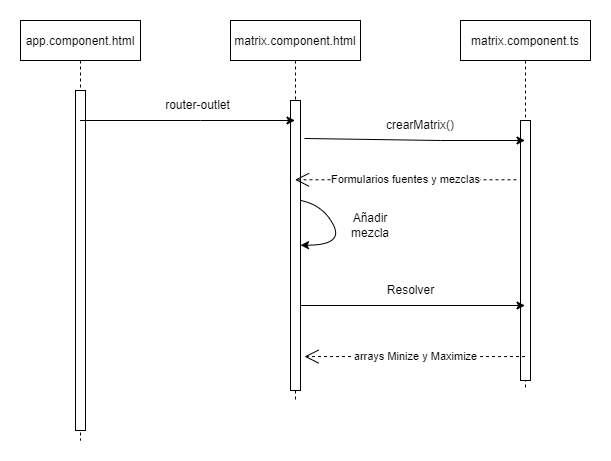
\includegraphics[width=1\textwidth]{img/flujo_01.drawio.png}
\caption{Flujo-01}
\label{fig:flujo_01}
\end{figure}

\newpage
\subsubsection{Flujo-02}

En este segundo flujo partimos del estado donde termino el flujo de la figura \ref{fig:flujo_01}, el cual es justo cuando el usuario visualiza la solución. Justo debajo de la solución se podrían encontrar dos botones ``Exportar problema' y ``Exportar solución''. El primero activa la función \textbf{exportProblem()} que genera un documento con los datos de entrada y llama a un componente de angular encargado de generar el archivo a descargar en el navegador. Este proceso es repetido de la misma forma al pulsar ``Exportar solución'', aunque añadiendo los datos de los arrays solución. Por último el usuario puede hacer click sobre cualquiera de los números de la solución y esto provocara una llamada a la función \textbf{download()} que genera un documento con la resolución de los pasos intermedios y este es descargado en el propio navegador al igual que los documentos anteriores.

\begin{figure}[h!] 
\centering
    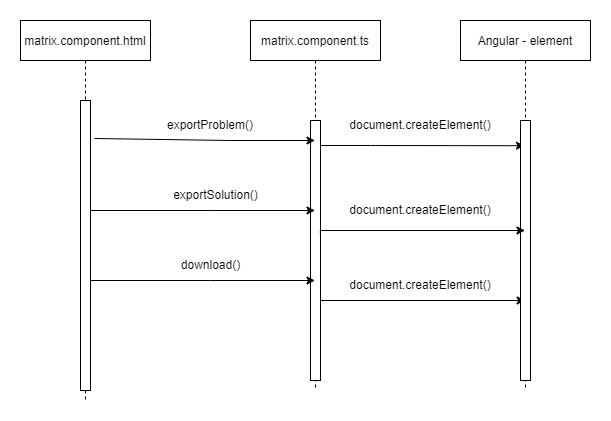
\includegraphics[width=1\textwidth]{img/flujo_02.drawio.png}
\caption{Flujo-02}
\label{fig:flujo_02}
\end{figure}

\subsubsection{Flujo cambio idioma - traducciones}

En este flujo hemos realizado el procedimiento llevado por la aplicación para realizar el cambio de idioma de las traducciones. Partimos de cualquier estado ya que el menú superior siempre está presente en la aplicación. Por tanto en el momento que cambia el select al otro idioma disponible se lanza un evento de cambio \textit{changeLang(event.target())} este evento cambia una variable ubicada en el local storage de la aplicación y toma como valor el seleccionado por el usuario. Esto hace que al realizar las traducciones tome el fichero correspondiente al idioma marcado \textit{assets/i18n/es.json} o \textit{assets/i18n/en.json}. 

\begin{figure}[h!] 
\centering
    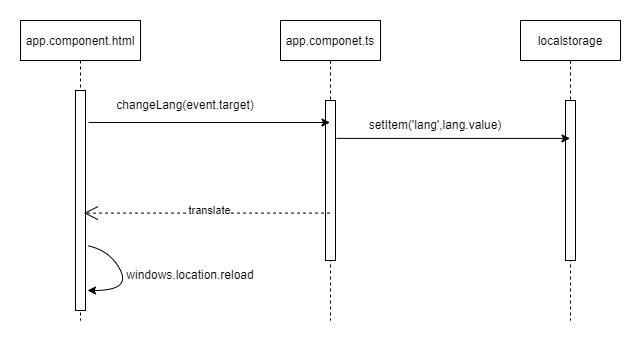
\includegraphics[width=1\textwidth]{img/traducciones.drawio.png}
\caption{Flujo traducciones}
\label{fig:flujo_traduc}
\end{figure}

\newpage
\section{Diseño arquitectónico}

Para realizar la arquitectura funcional de la aplicación se ha utilizado Angular, que una de sus características es que permite la creación de páginas tipo Single Page Application  (SPA). Se ha desarrollado el código siguiendo el patrón de diseño MVVM que divide la estructura del código en dos claras partes modelo y vista. En angular nos encontramos con dos tipos de archivos .ts encargándose de la lógica y las operaciones, y .html junto a .css encargados de la vista. 

El proyecto de angular está dividido en componentes que están formados por:

\begin{itemize}
    \item \textbf{Archivo .ts}: Vendría a ser el ``Modelo'' y contendría los datos a los que se accede desde la vista, además de métodos que modifican esos datos. La propiedad \textit{"two way binding"} hace un enlace bidireccional permitiendo a los componentes de la aplicación compartir datos, permitiendo escuchar eventos y actualizar valores simultáneamente.
    \item \textbf{Archivo .html}: Junto a el archivo .css que aporta los estilos formarían la "Vista" de la aplicación, presentando al usuario los datos en una interfaz fácil de entender.
\end{itemize}

\subsubsection{Servicios}

Un Servicio o \textit{Service} es una clase, comúnmente decorada con el decorador Injector de Angular, que indica que el Servicio puede inyectar otras dependencias de la aplicación, ya sean otros servicios como Http o hacer consultas AJAX.

\subsubsection{Módulos}

Los NgModules son contenedores para un bloque cohesivo de código dedicado al dominio de la aplicación, un flujo de trabajo o importaciones de librerías. Puede contener componentes, proveedores de servicios y otros archivos. Estos modulos se suelen dividir en las mismas partes: \textit{declarations}, \textit{imports}, \textit{exports} y \textit{providers}.




\apendice{Documentación técnica de programación}

\section{Introducción}

En este apéndice se detallan aspectos relacionados a la documentación técnica. Se describirá la estructura de directorios, un apartado dedicado al montaje de desarrollo con el cual se ha trabajo, y un último apartado, dedicado a pruebas del sistema.

\section{Estructura de directorios}

La estructura de directorios (ver figura \ref{fig:estructura_github}) del repositorio GitHub contienen la aplicación web, la API y la documentación del trabajo.

\begin{figure}[h!] 
\centering
    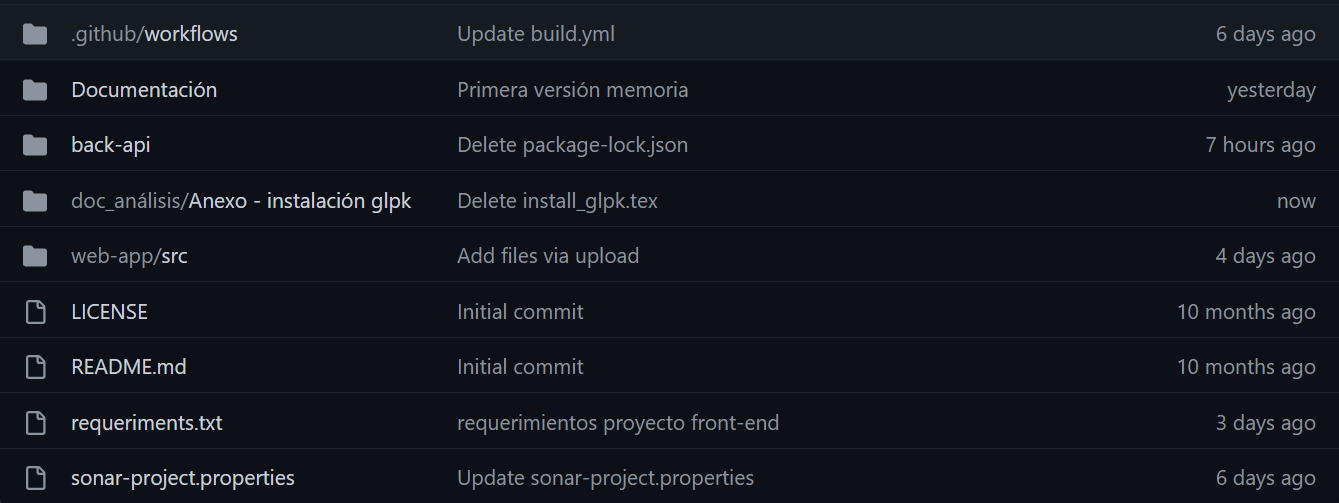
\includegraphics[width=0.8\textwidth]{img/estructura_github.PNG}
\caption{Estructura directorios, repositorio GitHub}
\label{fig:estructura_github}
\end{figure}

\subsection{.github.workflows}

Contiene archivos de configuración para el análisis de los códigos desde la herramienta Sonarcloud.

\subsection{Documentación}

Este directorio contiene los documentos de la memoria y los anexos. Así como los archivos .tex y las imágenes que forman los documentos.

\subsection{back-api}

Carpeta contiene el código de la API, que es un proyecto Laravel. Es importante destacar que este documento \textbf{no se ha usado en la parte de la subida al servidor}. Debido a problemas con la instalación de la librería GLPK \cite{glpk:package}. Pero hemos querido añadirlo, ya que ha sido un proyecto que ha servido como aprendizaje sobre como se comunican un proyecto front con un back.


\subsection{doc\_análisis}

Carpeta contiene documentos de análisis en \LaTeX. Algunas partes de estos documentos se han añadido a la memoria. Pero en su mayoría su objetivo ha sido documentar algunas lecturas interesantes del proceso de aprendizaje de herramientas. Y realizar algún documento de práctica con la nomenclatura de \LaTeX.


\subsection{web-app}

En este directorio hemos subido el contenido de la carpeta \textbf{src} del proyecto Angular. En la figura \ref{fig:src_angular} podemos ver los directorios default que tiene cualquier proyecto de angular.

\begin{figure}[h!] 
\centering
    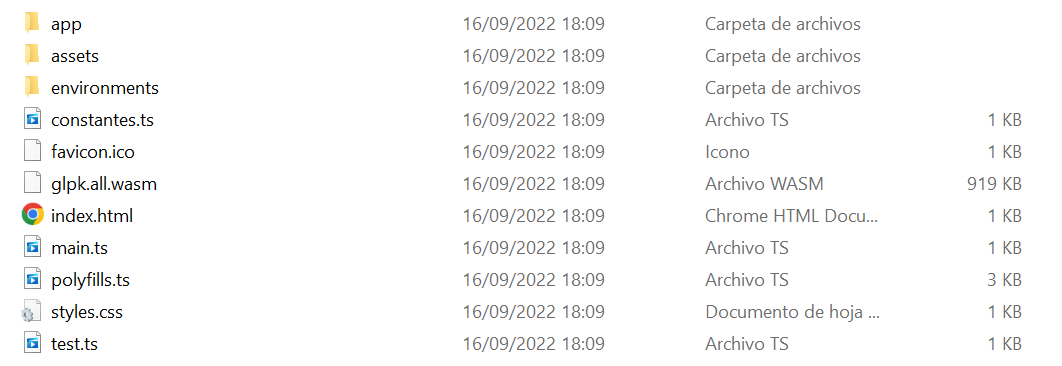
\includegraphics[width=0.8\textwidth]{img/src_angular.PNG}
\caption{Estructura directorio web-app/src}
\label{fig:src_angular}
\end{figure}

\begin{itemize}
    \item \textbf{Directorio app:} index.html es la página que contiene los componentes de las aplicaciones Angular. Estos componentes se encuentran dentro del directorio app (ver figura \ref{fig:app_angular}).
    
    \begin{figure}[h!] 
    \centering
        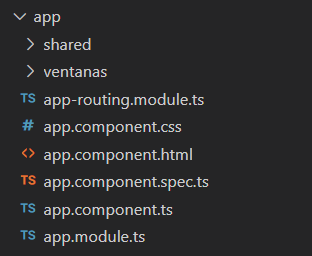
\includegraphics[width=0.8\textwidth]{img/app_angular.PNG}
    \caption{Estructura directorio web-app/src/app}
    \label{fig:app_angular}
    \end{figure}
    
    \newpage
    Directorios incluidos:
    
        \begin{itemize}
            \item \textbf{app-routing.module.ts:} contiene las rutas de la aplicación, están asignadas a componentes o módulos
            \item \textbf{app.component.css:} hoja de estilos del archivo \textit{app.component.html}
            \item \textbf{app.component.html:} archivo con la vista de la aplicación, archivo al que se apunta desde \textit{index.html}.
            \item \textbf{app.component.spec.ts:} archivo de pruebas del componente \textit{AppComponent}, que es el componente inicial de la aplicación.
            \item \textbf{app.component.ts:} archivo incluye la lógica del componente de arranque.
            \item \textbf{app.module.ts: }contiene la configuración de los imports y exports de módulos y componentes.
            \item \textbf{carpeta shared: } se ha configurado como un módulo que contiene componentes comunes en toda la aplicación.
            \item \textbf{carpeta ventanas:} contiene los componentes de las rutas principales de la aplicación.
        \end{itemize}
    
    \item \textbf{Directorio assets:} es el encargado de almacenar elementos estáticos como imágenes, pdfs, archivos mp3, etc (ver figura \ref{fig:assets_angular}).
    
    \begin{figure}[h!] 
    \centering
        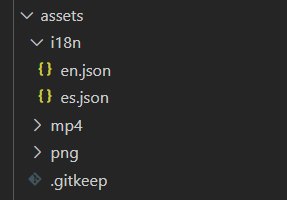
\includegraphics[width=0.8\textwidth]{img/assets_angular.PNG}
    \caption{Estructura directorio web-app/src/assets}
    \label{fig:assets_angular}
    \end{figure}
    
    \newpage
    Directorios incluidos:
    
    \begin{itemize}
        \item \textbf{Carpeta i18n:} contiene los archivos \textit{.json} con las traducciones tanto al inglés como al español.
        \item \textbf{Carpeta mp4:} contiene archivos con formato \textit{.mp4}, en este caso únicamente el vídeo guía de uso de la aplicación.
        \item \textbf{Carpeta png:} carpeta que contiene todas las imágenes e iconos usados en la aplicación
    \end{itemize}
    
    
    \item \textbf{Directorio environments:} nos permitir definir configuraciones para desplegar en un entorno local o producción.
    \item \textbf{constantes.ts:} archivo destinado a definir constantes globales para toda la aplicación.
    \item \textbf{favicon.ico:} es $16x16$ icon que sirve de icono de la web, permitiendo localizar al usuario la aplicación cuando se trabaja con múltiples ventanas
    \item \textbf{glpk.all.wasm:} archivo librería instalada GLPK.
    \item \textbf{index.html:} estructura inicial de documento HTML5; en este archivo se realiza la carga de scripts, estilos y dependencias necesarias. Además este archivo hace una llamada al fichero \textit{favicon.ico}
    \item \textbf{main.ts:} Este fichero es el encargado de definir qué módulo es el de arranque. Apuntando normalmente al AppComponent.
    \item \textbf{polyfills.ts:} Contiene algunos archivos para que nuestra aplicación sea compatible con algunos navegadores antiguos. El código se transpila a ES6 que no es compatible con algunas versiones de Internet Explorer o Firefox (ES5 si que es compatible) 
    \item \textbf{styles.css:} hoja de estilos asociada al archivo \textit{index.html}. Es llamado desde el archivo \textit{angular.json} configurándolo como la hoja principal de estilos de la aplicación.
    \item \textbf{test.ts:} Define la configuración que va a utilizar Karma. En este archivo se define el entorno de prueba.
\end{itemize}

\subsection{Ficheros adicionales}

\begin{itemize}
    \item \textbf{LICENSE:} archivo contiene información referente a la licencia marcada en el repositorio.
    \item \textbf{README.md:} Archivo presentación del repositorio GitHub y del proyecto.
    \item \textbf{requeriments.txt:} contiene parte del archivo \textbf{package.json} del proyecto en Angular. Está formado por las dependencias de la aplicación, y se usa en el proceso de montaje del proyecto. 
    \item \textbf{sonar-project.properties:} archivo de configuración de SonarCloud en el repositorio
\end{itemize}

\section{Manual del programador}

En esta sección se va a realizar la configuración de un entorno de desarrollo con las herramientas principales con las que se ha trabajado.

\subsubsection{Instalación Visual Studio Code}

Visual Studio Code se ha usado como framework de desarrollo. Se puede descargar mediante en enlace \url{https://code.visualstudio.com/download}, donde podremos descargar la versión correspondiente a nuestro sistema operativo.

Algunas de las extensiones que hemos utilizado en el desarrollo son (figura \ref{fig:visualstudio_extensions}):

\begin{figure}[h!] 
\centering
    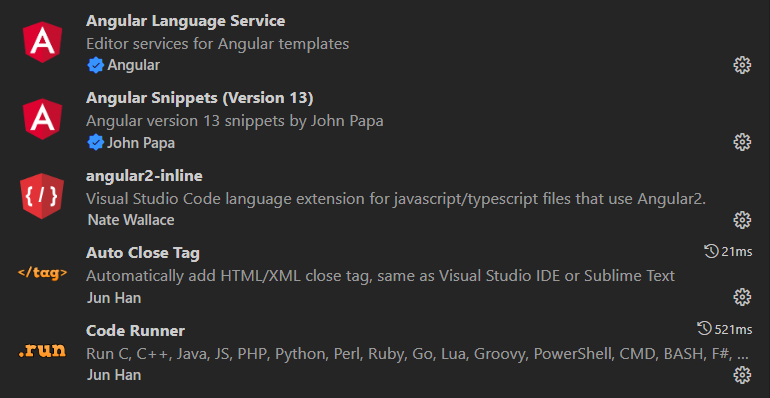
\includegraphics[width=1\textwidth]{img/visualcode_extensiones.PNG}
\caption{Visual Studio Code extensiones}
\label{fig:visualstudio_extensions}
\end{figure}

\subsubsection{Instalación Postman}

Para ejecutar las pruebas funcionales de la API, hemos utilizado la herramienta Postman que se puede descargar en el siguiente link de descarga: \url{https://www.postman.com/downloads/}

\subsubsection{Instalación Nodejs y npm}

Para el proyecto angular es necesario tener una versión de Nodejs instalada. Podemos obtener este link de descarga en su página oficial: \url{https://nodejs.org/es/download/}, seleccionando la versión dependiendo nuestro sistema. Después de la instalación es recomendable reiniciar el equipo.

\subsubsection{Instalación Debian}

Hemos usado Debian para simular un subsistema Linux en un sistema principal Windows. Link de descarga en: \url{https://apps.microsoft.com/store/detail/debian/9MSVKQC78PK6?hl=es-es&gl=es}


\section{Compilación, instalación y ejecución del proyecto}

Para utilizar el proyecto es necesario dirigirse al Github en \url{https://github.com/humbertoms99/Mixing_models}, y descargar el zip del repositorio.

\subsection{Instalación Angular y librerías Node}

Previamente debemos tener instalado Nodejs, ya que vamos a necesitar ejecutar algunos comandos npm.

Nos posicionamos en la ruta donde queremos montar el proyecto y ejecutamos el comando \textit{npm install -g @angular/cli} que instalará las dependencias angular/cli.
Creamos un proyecto angular \textit{ng new mixing\_models} (ver figura \ref{fig:ng_new}), y entramos en la carpeta creada con \textit{cd mixing\_models}. El siguiente paso es instalar las librerías (Recomendable hacerlo con la opción más abajo): \\


\begin{figure}[h!] 
\centering
    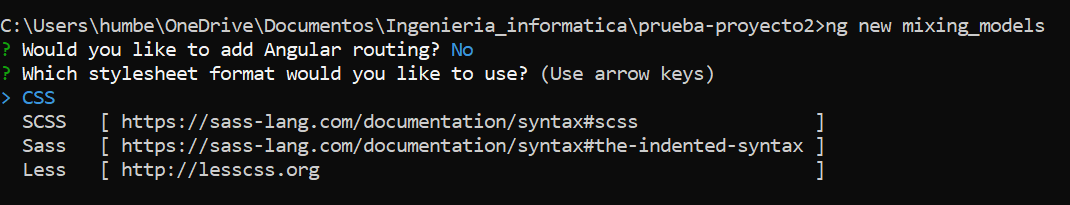
\includegraphics[width=0.8\textwidth]{img/ng_new.PNG}
\caption{Comando ng new nombre-proyecto}
\label{fig:ng_new}
\end{figure}

Instalación librería Fast Combinatorial Non-negative Least Squares:
$$ npm\:i\:ml-fcnnls $$
Instalación GLPK interface for TypeScript:
$$ npm\:install\:glpk-ts $$
Angular Material:
$$ ng\:add\:@angular/material  $$
Angular ngx-translate:
$$ npm\:install\:@ngx-translate/core\:@ngx-translate/http-loader $$
GLPK compiled to wasm:
$$ npm\:i\:glpk-wasm $$
Y los comandos:
$$ npm\:install\:@types/node\:--save-dev $$
$$ npm\:install\:@angular/localize\:--save $$

En vez de realizar estas instalaciones podemos abrir el archivo \textbf{package.json} y copiar el contenido de la carpeta \textit{requeriment.txt} del GitHub. Y copiar de esta forma las dependencias del proyecto, y para instalarlas ejecutamos el comando:

$$ npm\:install\:--legacy-peer-deps $$

En el archivo \textbf{angular.json}: 

\begin{figure}[h!] 
\centering
    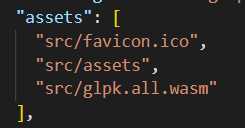
\includegraphics[width=0.8\textwidth]{img/angular_json.PNG}
\caption{Configuración angular - angular.json}
\label{fig:angular_json}
\end{figure}

En el archivo \textbf{tsconfig.json}: 

\begin{figure}[h!] 
\centering
    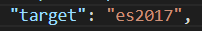
\includegraphics[width=0.8\textwidth]{img/tsconfig_json.PNG}
\caption{Configuración angular - tsconfig.json}
\label{fig:tsconfig_json}
\end{figure}

\newpage
El el archivo \textbf{tsconfig.app.json}

\begin{figure}[h!] 
\centering
    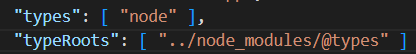
\includegraphics[width=0.8\textwidth]{img/tsconfig_app_json.PNG}
\caption{Configuración angular - tsconfig.app.json}
\label{fig:tsconfig_app_json}
\end{figure}

Por último, \textbf{borramos la carpeta src} y pegamos la carpeta src  que se encuentra dentro la carpeta web-app del zip descargado del repositorio del GitHub.

\subsection{Ejecución del proyecto}

Una vez configurado el proyecto, abrimos la terminal y nos posiciones en path del carpeta del proyecto con el comando:



Y para ejecutar la aplicación:

$$ ng\:serve\:-o $$

Con este comando no abrirá automáticamente una ventana en nuestro navegador, con la dirección \textit{http://localhost:4200/} 



\section{Pruebas del sistema}

Las pruebas de sistema validan el sistema completo y totalmente integrado. El objetivo de las pruebas de sistema es evaluar las especificaciones del sistema en su totalidad.

Para realizar estas pruebas hemos utilizado la herramienta SonarCloud que es una plataforma para evaluar la calidad del código fuentes. Es una herramienta de software libre y está vinculada con GitHub para obtener métricas de calidad de código.

Para poder realizar los análisis se han añadido los archivos \textit{sonar-project.properties} y \textit{.github/workflows/build.yml} y una key en el apartado de configuración del respositorio de GitHub. Esto hace que Sonarcloud analicé el contenido actual de la carpeta del proyecto Github.

Podemos ver el resumen del análisis del código en la figura \ref{fig:sonarcloud_res}. 

\begin{figure}[h!] 
\centering
    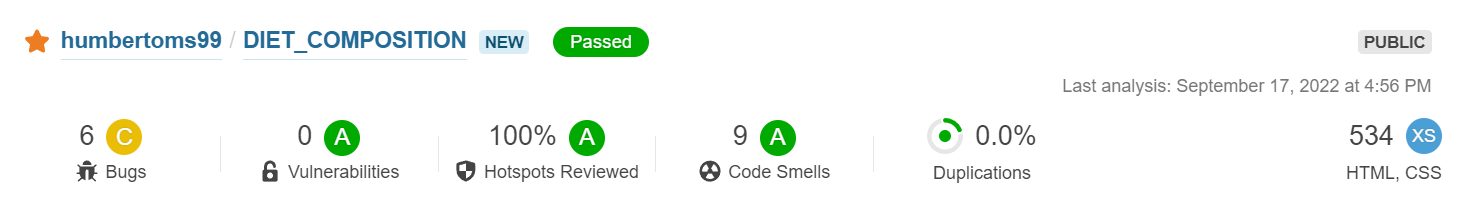
\includegraphics[width=1\textwidth]{img/sonarcloud_res_1.PNG}
\caption{Resumen análisis código Sonarcloud}
\label{fig:sonarcloud_res}
\end{figure}

\begin{itemize}
    \item \textbf{Bugs:} errores de código que pueden romper el código y deben ser corregidos cuando antes. 
    \item \textbf{Vulnerabilities:} partes del código que pueden ser explotadas por un hacker.
    \item \textbf{CodeSmells: } códigos que son confusos, y por tanto difíciles de mantener.
    \item \textbf{Security Hotspots: } código sensible a la seguridad que requiere una revisión manual para evaluar si existe o no una vulnerabilidad.
    \item \textbf{Duplications:} porcentaje de códigos duplicados en las nuevas líneas
    \item \textbf{Líneas de códigos y lenguajes utilizados.}
\end{itemize}

Además si accedemos a una rama concreta podemos ver análisis más específicos, como por ejemplo el listado de issues (figura \ref{fig:sonarcloud_issues}). Consideramos muy útil este apartado porque aparte de ofrecernos el listado completo de fallos pendientes por arreglar, nos da una aproximación de tiempo de cada issue y un tiempo total aproximado para todas, establece importancia y permite añadir etiquetas. Además permite asignar estas tareas al estar sincronizado con GitHub.

\begin{figure}[h!] 
\centering
    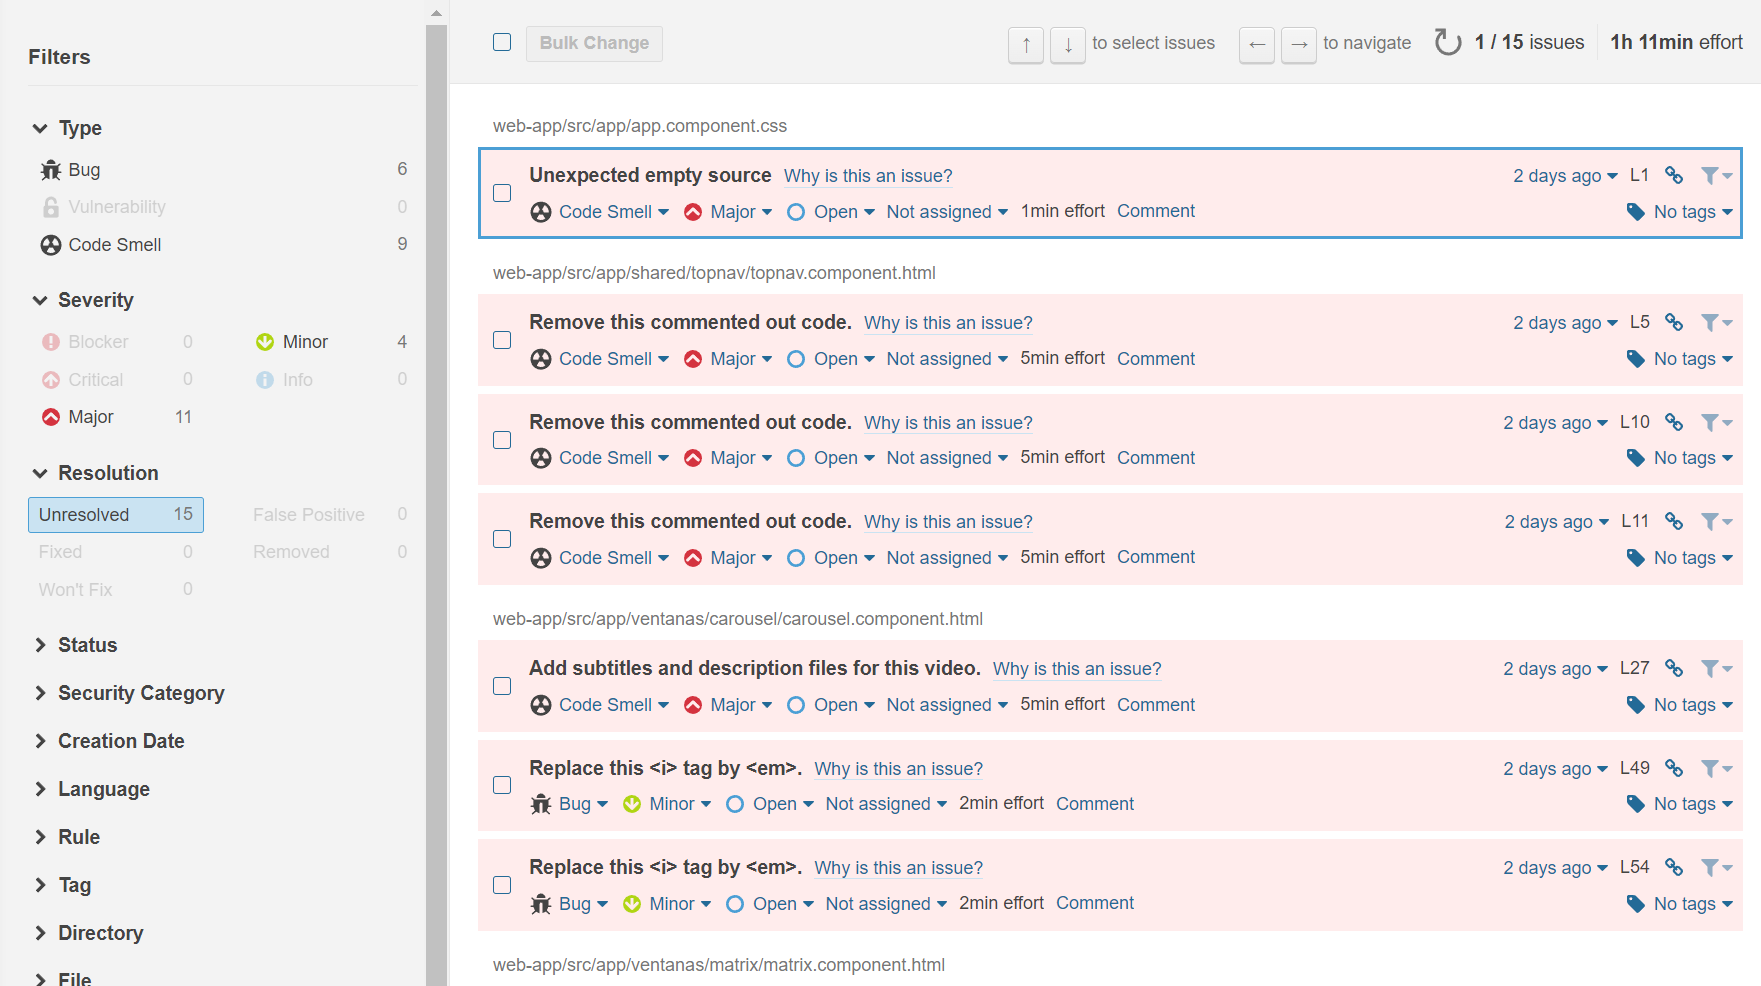
\includegraphics[width=1\textwidth]{img/sonarcloud_issues_1.PNG}
\caption{Sonarcloud issues brand main}
\label{fig:sonarcloud_issues}
\end{figure}

\newpage
Por último, podemos entrar al apartado de \textbf{Code} (ver figura \ref{fig:sonarcloud_lines_code}). En este apartado veremos un listado de todos los archivos, sus líneas de código y los Bugs, vulnerabilities, Code Smells, Security Hotspots, Coverage y Duplications. Apartado que puede servir para ver una visión general del código. 

\begin{figure}[h!] 
\centering
    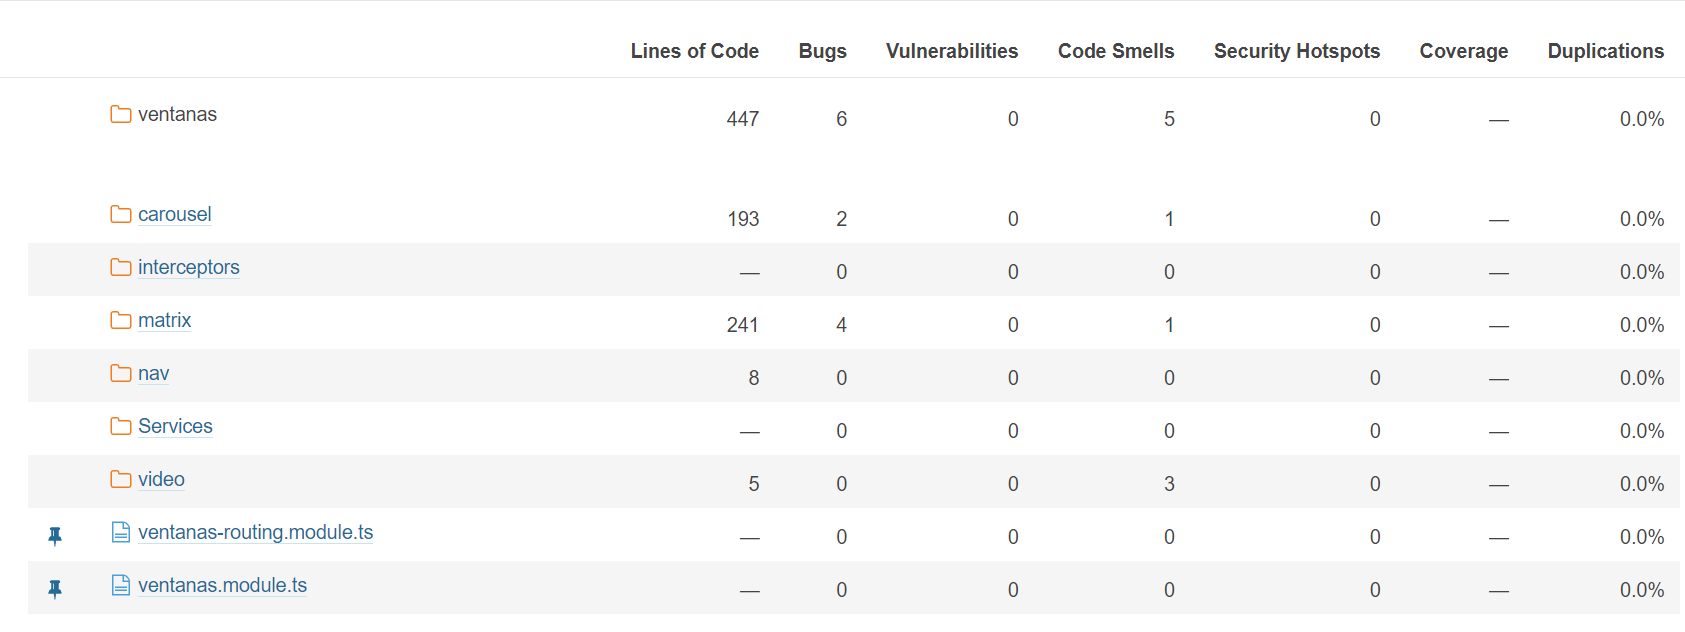
\includegraphics[width=1\textwidth]{img/sonarcloud_lines_code_1.PNG}
\caption{Sonarcloud líneas de código}
\label{fig:sonarcloud_lines_code}
\end{figure}



\apendice{Documentación de usuario}

\section{Introducción}

En este apéndice se detallan los requisitos para acceder al proyecto por parte de un usuario. Además se han descrito las funcionalidades de la aplicación en un manual de usuario.

\section{Requisitos de usuarios}

Al ser una aplicación web únicamente es necesario tener un navegador web y acceder mediante el enlace \url{https://mixingmodels.netlify.app/}. Por otra parte si se quiere poder ver el contenido .csv, se requiere alguna herramienta de lectura de hojas de cálculo.

\section{Instalación}

No requiere ninguna instalación.

\section{Manual del usuario}

Esta sección es dedicada a un apartado de guía de usuario, orientando a las personas que utilicen la web, ofreciendo asistencias a los usuarios y recopilando todas las funcionalidades que ofrece.

\subsubsection{Menú superior}

En la parte de superior de la pantalla encontramos un menú superior \ref{fig:topnav} que organiza la web en algunos apartados:

\begin{figure}[h!] 
\centering
    
\includegraphics[width=1\textwidth]{img/menu_sup.PNG}
\caption{Top Navigation Bar}
\label{fig:topnav}
\end{figure}

\begin{enumerate}
    \item \textbf{Problema:} vista principal contiene la resolución de problemas de sistemas ecuaciones con restricciones, recepción y exportación de datos. 
    \item \textbf{Video:} vista contiene un vídeo guía, que permite ver las principales funcionalidades de la aplicación al usuario aportando un ejemplo básico de resolución.
    \item \textbf{Icono GitHub:} enlace directo al repositorio GitHub, que contiene el código de la aplicación y documentación del proyecto.
    \item \textbf{About us:} desplegable que muestra los desarrolladores del proyecto.
    \item \textbf{Select de traducciones:} seleccionable que nos permite cambiar entre los dos idiomas de la aplicación Ingles y Español, únicamente dando click en al idioma que queramos cambiar.
\end{enumerate}

\subsubsection{Ventana resolución problema}

En esta ventana vemos la barra de navegación superior, y el contenido de la aplicación. El funcionamiento de la web es que según se introducen datos y se va creando la estructura del problema a resolver, se van desbloqueando apartados, terminando el último con la solución del problema y los botones de exportar.

En la Figura \ref{fig:ventana_inicial} aparece el primer formulario de la aplicación, destinado a marcar el tamaño de la matriz de fuentes de datos. Es importante recalcar que el botón \textit{``Crear''} no se activa mientras los valores de marcadores y fuentes sean inferiores o iguales a cero. Una vez rellenemos el formulario con valores válidos se habilitara el botón. Por otra parte disponemos de un botón adicional (Figura \ref{fig:importPlant}) que permite al usuario cargar una plantilla de datos. Esta parte se comentará en profundidad más adelante analizando la plantilla que requiere la aplicación.


\begin{figure}[h!] 
\centering
    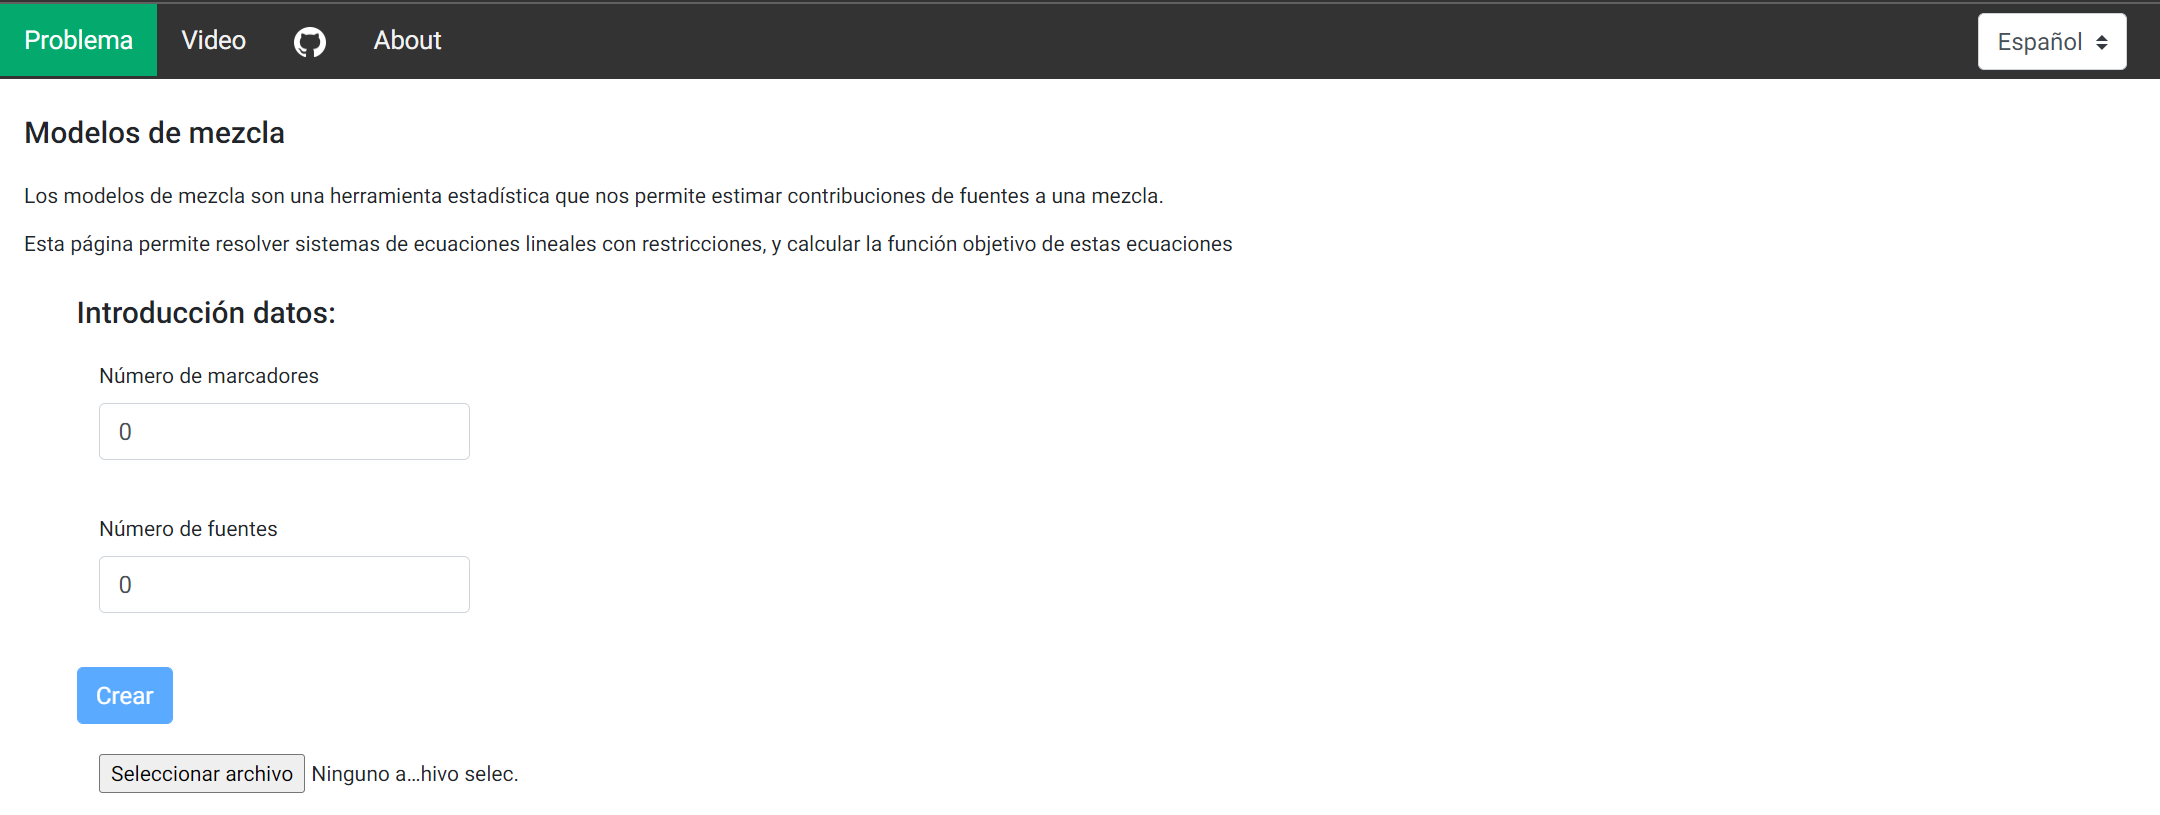
\includegraphics[width=1\textwidth]{img/ventana_inicial.PNG}
\caption{Ventana inicial web}
\label{fig:ventana_inicial}
\end{figure}

Una vez se habilita y pulsamos \textit{``Crear''}, muestra un nuevo formulario (Figura \ref{fig:data_matrix}). Siendo una matriz del tamaño fijado en el primer formulario, las filas son el número de fuentes y las columnas el número de marcadores. Se permite la introducción con números decimales, y para marcar la coma decimal se realiza con ".". Por otra parte, se ha añadido la opción de nombrar a las fuentes según queramos ofreciendo más personalización al problema.

\begin{figure}[h!] 
\centering
    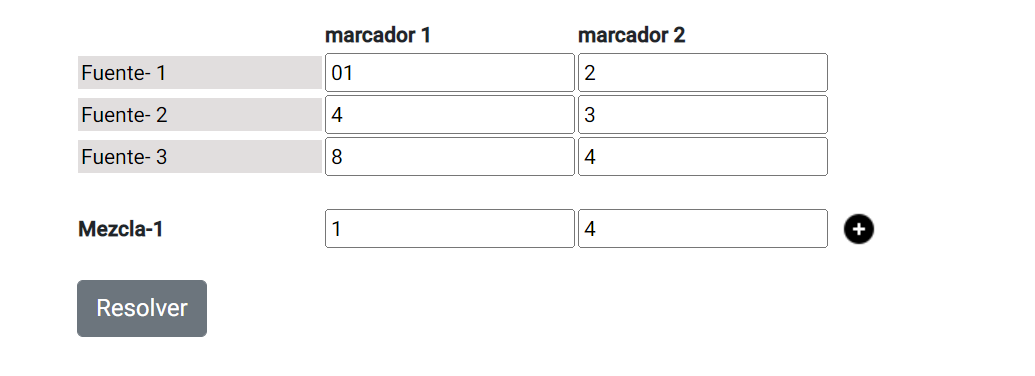
\includegraphics[width=1\textwidth]{img/datos_matriz.PNG}
\caption{Inputs datos matriz de fuentes}
\label{fig:data_matrix}
\end{figure}

En la parte inferior se encuentra la introducción de datos de las mezclas, teniendo estas el mismo número de marcadores que las fuentes. Inicialmente se encuentran datos de entrada para una única mezcla, pero podemos añadir con el botón situado a su derecha en la figura \ref{fig:data_matrix}, al pulsar, crea una nueva mezcla con el mismo tamaño de marcadores que el resto. 

Una vez hemos configurado la matriz de datos de entrada tanto de fuentes como de mezclas damos a \textit{``Resolver''}. En este momento se ejecuta una función que primero calcula las proyecciones de las mezclas respecto al plano de las fuentes y posteriormente se usa la librería GLPK para resolver el sistema. El ejercicio resuelve el sistema de ecuaciones con la restricción de que todas las $x$ cantidades deben ser superiores a $0$, esto es porque no se puede tener negativos de una cantidad. 

Por último se muestra la solución del sistema de ecuaciones mostrando las cantidades mínimas y máximas que pueden tener las fuentes respecto a las mezclas (Figura \ref{fig:sols_arrays}).

\begin{figure}[h!] 
\centering
    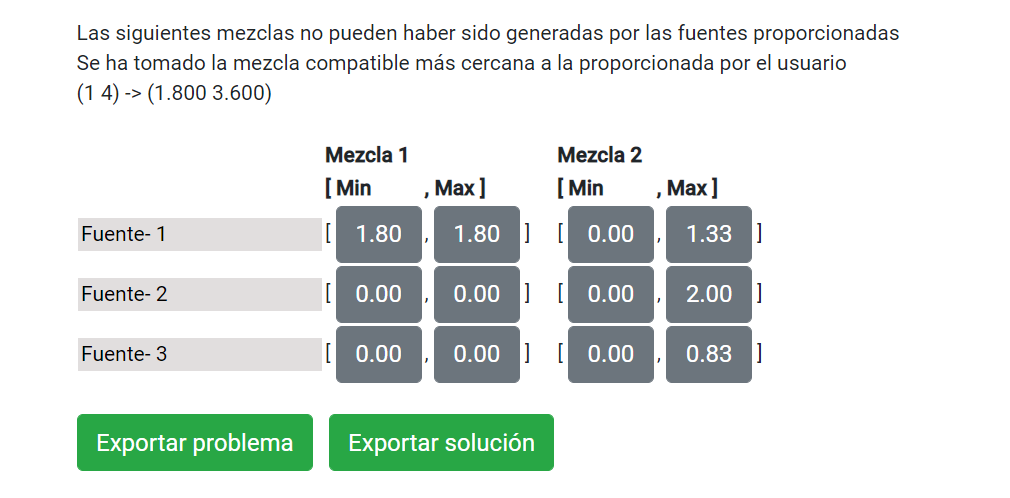
\includegraphics[width=1\textwidth]{img/solution_visual.PNG}
\caption{Arrays solución máximos y mínimos}
\label{fig:sols_arrays}
\end{figure}

En caso de que los \textit{"puntos mezclas"} se encuentre fuera del plano de fuentes, en una primera parte nos mostrará las proyecciones, las cuales son los valores utilizados en la resolución del sistema. 

Justo debajo de las proyecciones encontramos los arrays de solución de mínimos y máximos para cada mezcla sobre las fuentes. En la figura \ref{fig:sols_arrays} vemos entonces que la \textit{Fuente-1} tendría una proporción mínima de $1.80$ y una máxima de $1.80$ sobre la \textit{Mezcla 1}, y una proporción mínima de $0.00$ y una máxima de $1.33$ sobre la \textit{Mezcla 2}, comentar que estos valores solución se han redondeado a dos decimales y las proyecciones a tres.

Una vez hemos resuelto el ejercicio, la aplicación ofrece diferentes opciones de exportar los datos de la solución, a continuación veremos las tres posibilidades:

\textbf{Exportar problema: } en la figura \ref{fig:sols_arrays} si presionamos \textit{``Exportar problema''} nos descarga un archivo con nombre \textit{``InputData.csv''} que contiene los datos de la figura \ref{fig:inputData}. Manteniendo siempre la misma estructura: las dos primeras filas marcan el tamaño de la matriz de datos \textbf{marcadores} y \textbf{fuentes}, una fila en blanco y justo debajo una fila por cada fuente que se haya especificado. Por último, dejando una línea de separación encontramos una fila para cada mezcla. 

El objetivo de este documento es servir como plantilla que permita cargar este mismo problema en futuros usos.

\begin{figure}[h!] 
\centering
    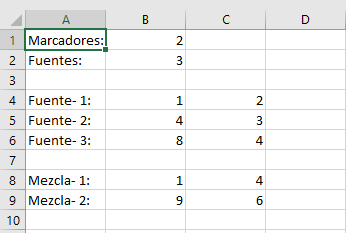
\includegraphics[width=1\textwidth]{img/inputData.PNG}
\caption{Export datos entrada problema}
\label{fig:inputData}
\end{figure}

\textbf{Exportar solución: } en la figura \ref{fig:sols_arrays} si presionamos \textit{``Exportar solución''} nos descarga un archivo de nombre \textit{"Solution.csv"}, que contiene la estructura de datos de la figura \ref{fig:solution}. El objetivo de este documento es tanto mostrar los datos de entrada como la solución del sistema, en las primeras filas encontramos el mismo diseño que con \textit{``Exportar problema''}. A continuación, se deja una línea en blanco y se muestra las proyecciones de las mezclas en caso de haberlas. Se deja otra fila en blanco y se muestra una estructura de tabla muy parecida a la visual de la web.

\begin{figure}[h!] 
\centering
    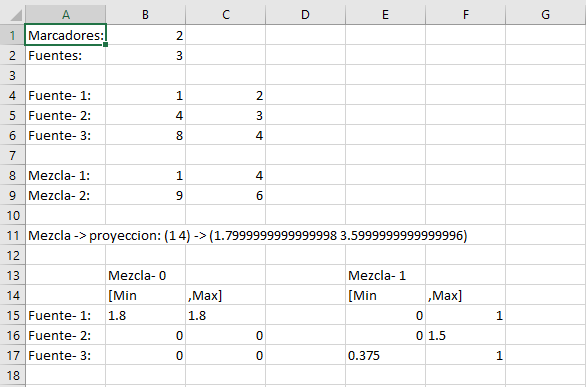
\includegraphics[width=1\textwidth]{img/solution.PNG}
\caption{Export solución completa}
\label{fig:solution}
\end{figure}

\textbf{Exportar pasos intermedios:} para descargar este documento podemos pulsar encima del número de la solución del cual queramos ver sus pasos intermedios, en el caso de la figura \ref{fig:pasoIntermedio} se ha pulsado sobre el valor $1.80$ de la \textit{Fuente-1} y \textit{Min} de la \textit{Mezcla-1}.

La estructura del documento está compuesta por unas primeras filas con restricciones del sistema, la función objetivo y las ecuaciones del sistema de ecuaciones.

\begin{figure}[h!] 
\centering
    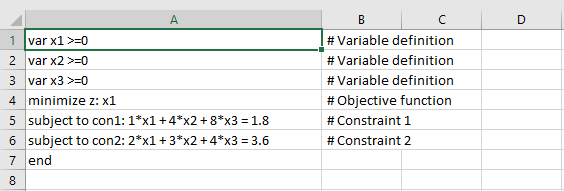
\includegraphics[width=1\textwidth]{img/pasoIntermedio.PNG}
\caption{Export resolución paso intermedio}
\label{fig:pasoIntermedio}
\end{figure}

A partir del documento de la figura \ref{fig:inputData} que funciona como plantilla de entrada podemos pulsar el botón \textit{"Seleccionar archivo"} de la figura \ref{fig:selectFile}. Esta acción abre el nuestro sistema de directorios (Figura \ref{fig:importPlant}) y podemos seleccionar la plantilla de datos exportada anteriormente. 

\begin{figure}[h!] 
\centering
    
\includegraphics[width=1\textwidth]{img/selectFile.PNG}
\caption{Botón seleccionar archivo}
\label{fig:selectFile}
\end{figure}

\begin{figure}[h!] 
\centering
    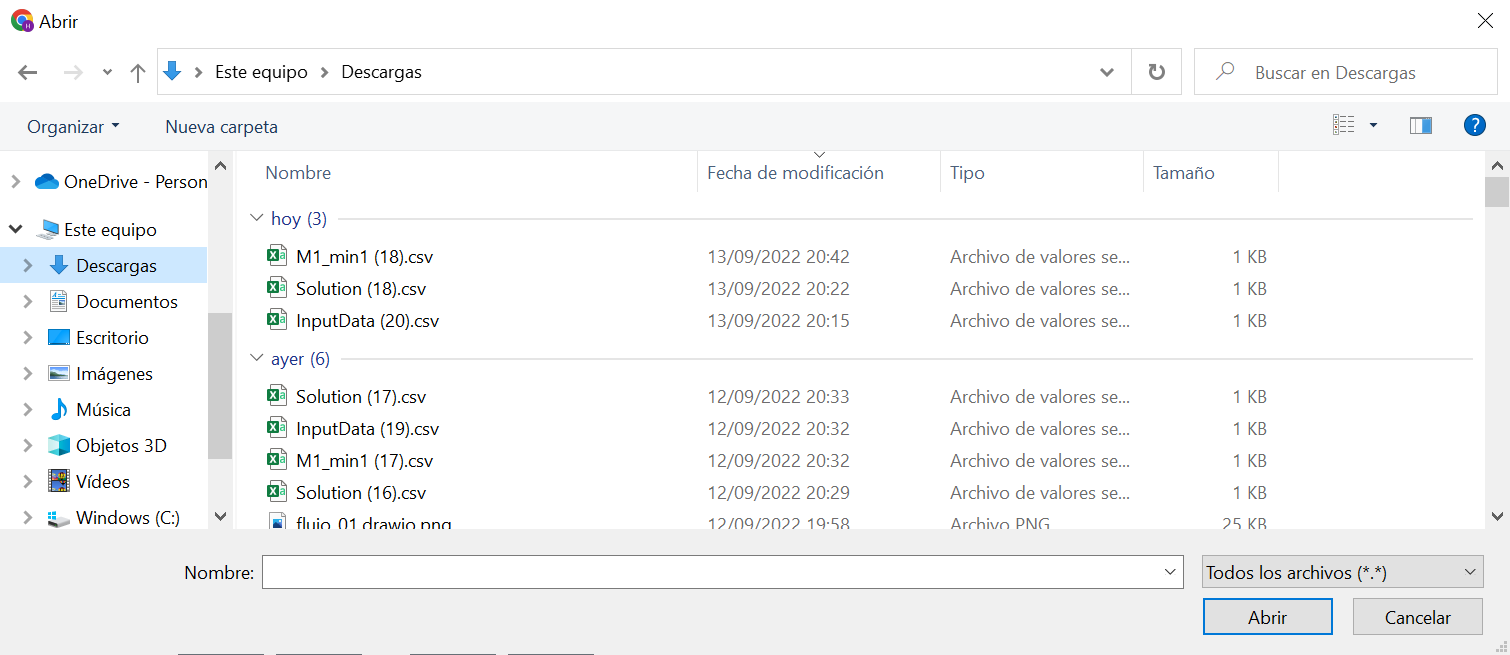
\includegraphics[width=1\textwidth]{img/directoryInport.PNG}
\caption{Importar plantilla}
\label{fig:importPlant}
\end{figure}

\newpage
El resultado de seleccionar una plantilla de datos es el de la figura \ref{fig:visualwebimport}, con la matriz de fuentes y mezclas con los valores y tamaños de la plantilla. Esto deja la aplicación justo antes de dar a \textit{``Resolver''}.

\begin{figure}[h!] 
\centering
    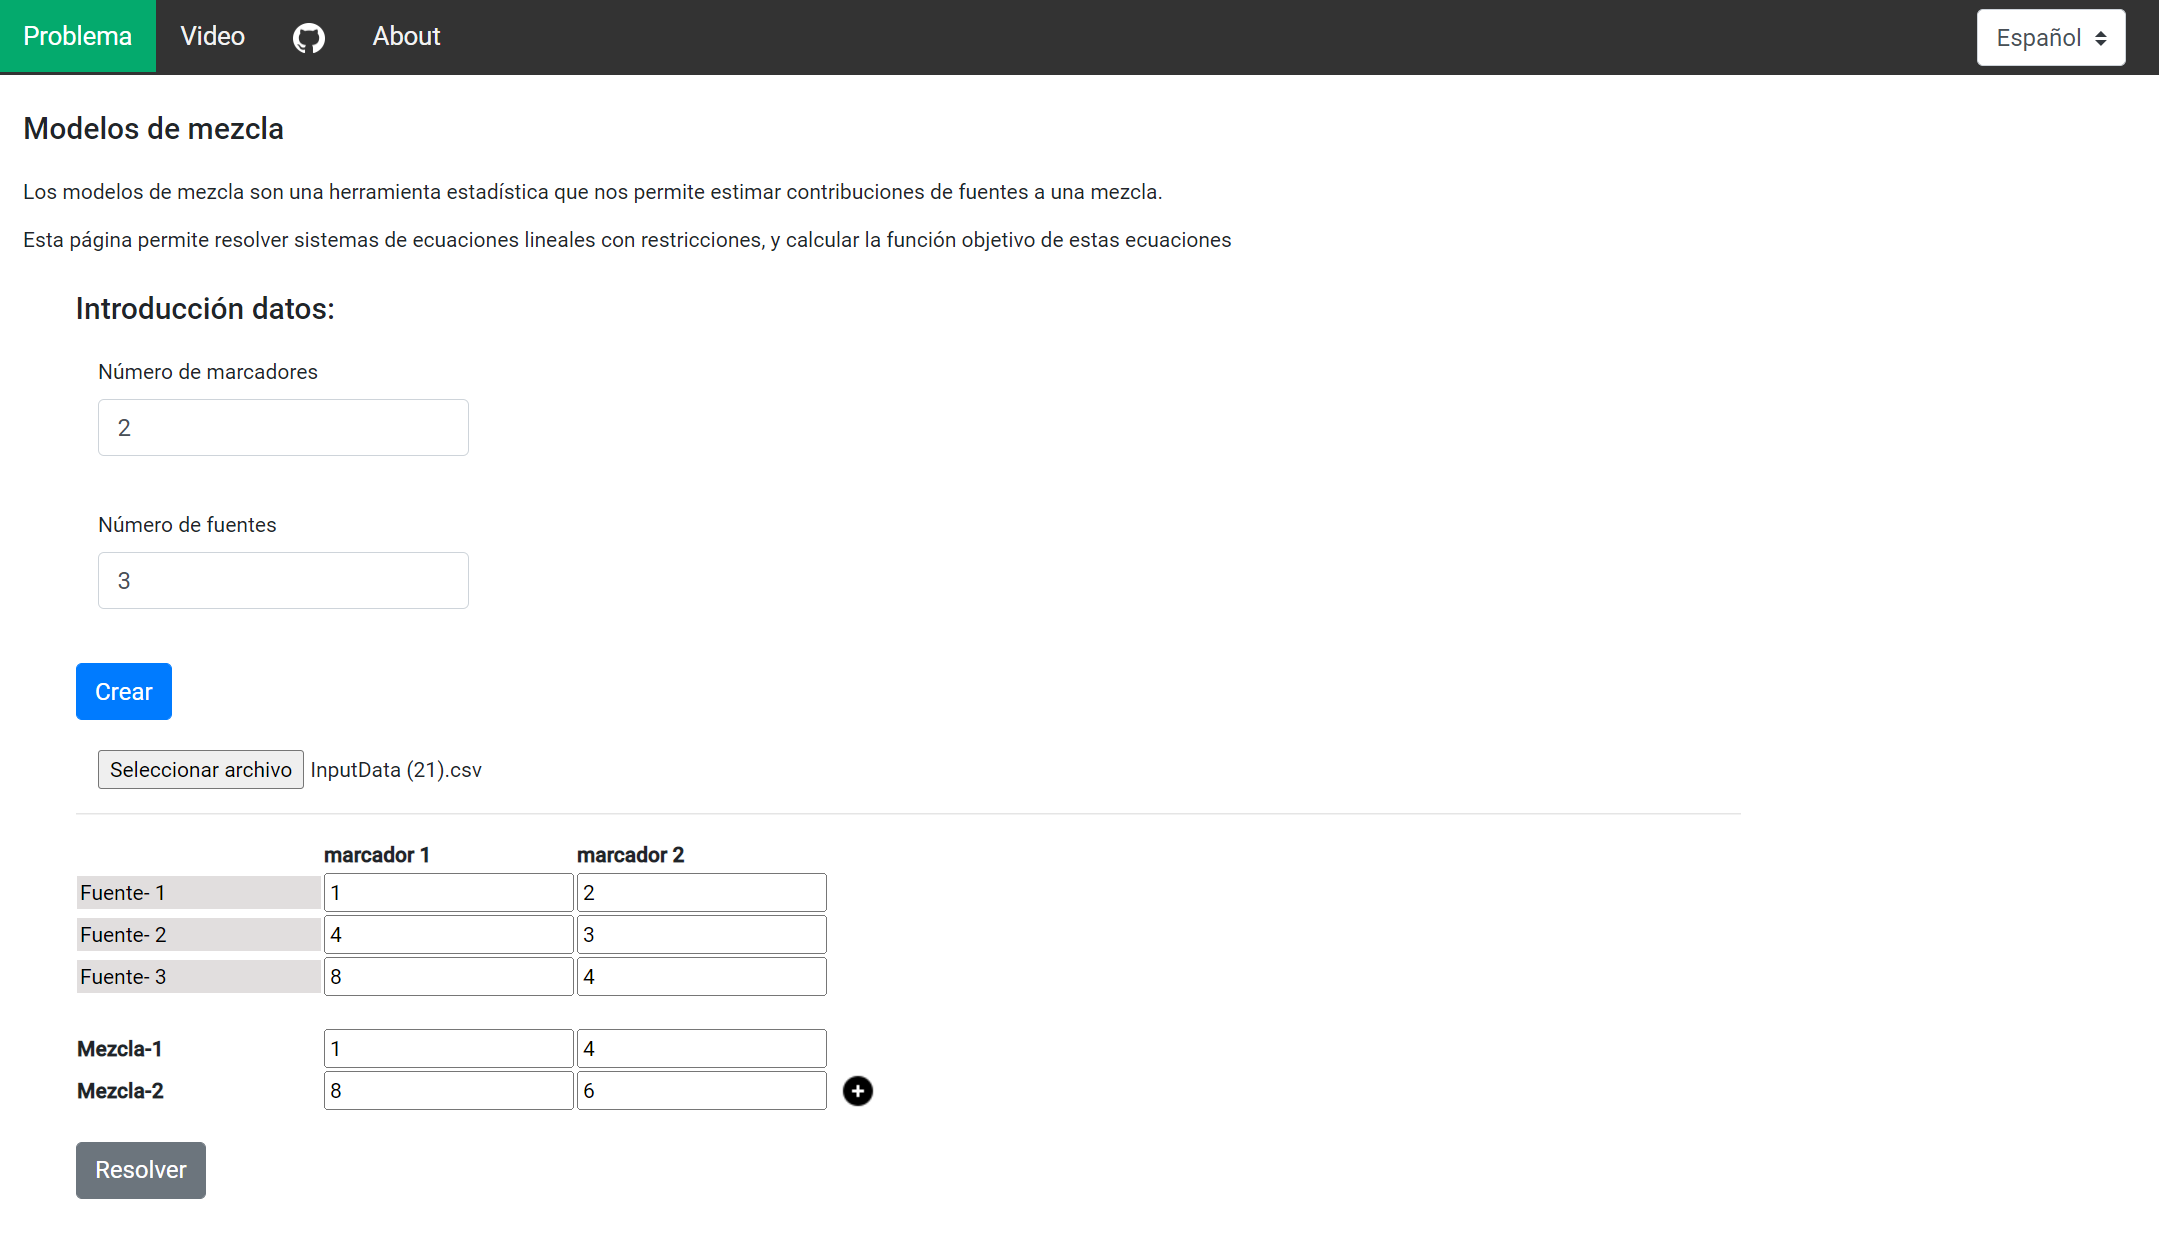
\includegraphics[width=1\textwidth]{img/importVisual.PNG}
\caption{Importar visual web}
\label{fig:visualwebimport}
\end{figure}


\bibliographystyle{plain}
\bibliography{bibliografiaAnexos}

\end{document}
